% указываем класс документа
%\documentclass[twoside,8pt,a5paper,openany]{report}
\documentclass[twoside,12pt,a4paper,openany]{report}

% подключаем собственный стилевой файл
\usepackage{labstyle}
\usepackage{labstyle2}







\makeindex





\begin{document}


% указываем язык (для автоматической вставки слов, типа "Глава", "Содержание", "Литература", "рис." и пр.
\selectlanguage{ukrainian}



% подключаем файлы содержимого
\begin{titlepage}
\newpage

\begin{center}
МІНІСТЕРСТВО ОСВІТИ І НАУКИ УКРАЇНИ \\

ХЕРСОНСЬКИЙ ПОЛІТЕХНІЧНИЙ КОЛЕДЖ \\

ОДЕСЬКОГО НАЦІОНАЛЬНОГО ПОЛІТЕХНІЧНОГО УНІВЕРСИТЕТУ\\

ВІДДІЛЕННЯ КОМП'ЮТЕРНОЇ ТА ПРОГРАМНОЇ ІНЖЕНЕРІЇ

\end{center}


\vspace{10em}

\begin{center}
\Large Курс лекції \\ з дисципліни
\end{center}

\vspace{2em}

\begin{center}
\huge{\textbf{<<Алгоритми та структури даних>>}}
\end{center}




\vspace{\fill}

\begin{center}
Херсон --- 2015
\end{center}

\end{titlepage}



% ненужное можно просто закомментировать знаком процента "%" 

% первую страницу не нумеруем
%\thispagestyle{empty}			

% название
%\title{Методичні вказівки до лабораторних робіт з дисципліни <<web-програмування>>}
%\author{Жарікова М.В., Левицький В.М.}
%\maketitle

% печатаем содержание
%\chapter*[Зміст]{Зміст}
\tableofcontents

% ничанаем с новой страницы
%\newpage

% печатаем перечень рисунков
%\chapter*{Перелік ілюстрацій}
\listoffigures

% печатаем перечень таблиц
%\chapter*{Перелік таблиць}
\listoftables

\lstlistoflistings

%\lstlistoflistings


\chapter{Рекурсія}
\nopagebreak[4]
\section*{Мета роботи}

\nopagebreak[4]
\section{Вступ}
\nopagebreak[4]
У математиці для вирішення переважної більшості завдань використовуються методи, які в кінцевому рахунку можуть бути зведені до одного з двох базових способів: ітерації або рекурсії.


\textbf{Ітерація} означає кількаразове повторення одних і тих же дій, яке після деякої кількості кроків приводить до бажаного результату. Характерним прикладом ітераційного способу вирішення завдання є методи послідовних наближень рішення нелінійних рівнянь, у тому числі метод дотичних, метод хорд і т.д.

\begin{equation}
f(x)=0; x=\varphi(x); x_0=a; x_n=\varphi(x_{n-1}), n=1,2,..., |x_k-x_{k-1}|>\epsilon
\end{equation}

\textbf{Рекурсія} являє собою посилання при описі об'єкта, дії на описуваний об'єкт, дія. Рекурсія означає рішення задачі за допомогою відомості рішення до самого себе. При цьому обчислення залежать від інших, в не-якому сенсі більш простих (зазвичай менших) значень аргументу або аргументів завдання. Повністю аналогічні механізми використовуються в базовій теорії рекурсивних функцій, у методі математичної індукції, а також в рекурентних послідовностях. 

Наприклад:

\begin{equation}
a_k = 2a_{k-1} + k , \forall k > 0, a_0 = 1
\end{equation}

\textbf{Рекурсивний алгоритм} - це алгоритм, в описі якого прямо або побічно міститься звернення до самого себе. У техніці процедурного програмування дане поняття поширюється на функцію, яка реалізує рішення окремого блоку завдання за допомогою виклику зі свого тіла інших функцій, в тому числі і себе самої. Якщо при цьому на черговому етапі роботи функція організовує звернення до самої себе, то така функція є рекурсивної.



\section{Ключові терміни}
\nopagebreak[4]


\textbf{База рекурсії} - це тривіальний випадок, при якому рішення задачі очевидно, тобто не потрібно звернення функції до себе.

\textbf{Глибина рекурсивних викликів} - це найбільше одночасне кількість рекурсивних звернень функції, визначальне максимальну кількість шарів рекурсивного стека.

\textbf{Декомпозиція} - це вираження загального випадку через більш прості підзадачі зі зміненими параметрами.

\textbf{Корінь повного дерева рекурсивних викликів} - це вершина повного дерева рекурсії, відповідна початкового зверненням до функції.

\textbf{Непряма (взаємна) рекурсія} - це послідовність взаємних викликів декількох функцій, організована у вигляді циклічного замикання на тіло первісної функції, але з іншим набором параметрів.

\textbf{Обсяг рекурсії} - це характеристика складності рекурсивних обчислень для конкретного набору параметрів, що представляє собою кількість вершин повного рекурсивного дерева без одиниці.

\textbf{Параметризація} - це виділення з постановки задачі параметрів, які використовуються для опису умови задачі і рішення.

\textbf{Повне дерево рекурсії} - це граф, вершинами якого є набори фактичних параметрів при всіх викликах функції, починаючи з першого звернення до неї, а ребрами - пари таких наборів, відповідних взаємним викликам.

\textbf{Пряма рекурсія} - це безпосереднє звернення рекурсивної функції до себе, але з іншим набором вхідних даних.

\textbf{Рекурсивна тріада} - це етапи вирішення завдань рекурсивним методом.

\textbf{Рекурсивна функція} - це функція, яка у своєму тілі містить звернення до самої себе зі зміненим набором параметрів.

\textbf{Рекурсивний алгоритм} - це алгоритм, у визначенні якого міститься прямий або непрямий виклик цього ж алгоритму.

\textbf{Рекурсія} - це визначення об'єкта за допомогою посилання на себе.


\section{Розширені теоретичні відомості}
\nopagebreak[4]


Рекурсивні алгоритми зазвичай виходять на основі математичної постановки завдання. Найважливіше при побудові рекурсивного алгоритму: побачити однакові дії на поточному та попередньому кроці обчислень (дій).

Виконавець рекурсивного алгоритму зводить невідоме до іншого невідомого, накопичуючи інформацію (прямий хід) і відкладаючи фактичні обчислення до моменту, коли виконається умова, що дозволяють безпосередньо обчислити шукане значення. Потім виконується зворотний хід рекурсії.

\textbf{Основні переваги рекурсії:}
\begin{itemize}
\item простота математичного формулювання;
\item простота алгоритму і його реалізації
\end{itemize}
\textbf{Основні недоліки рекурсії:}
\begin{itemize}
\item додаткові витрати оперативної пам'яті;
\item додаткові тимчасові витрати;
\item можливий перехід складності в клас EXP.
\end{itemize}

За аналогією з математичної індукцією, на яку рекурсія трохи схожа, будь рекурсивна процедура повинна включати в себе базис і крок рекурсії.

Базис рекурсії - це пропозиція, що визначає якусь початкову ситуацію або ситуацію в момент припинення. Як правило, в цій пропозиції записується якийсь найпростіший випадок, при якому відповідь виходить відразу навіть без використання рекурсії. Так, у наведеній вище процедурі, яка описує предикат предок, базисом рекурсії є перше правило, в якому визначено, що найближчими предками людини є його батьки. Ця пропозиція часто містить умову, при виконанні якї відбувається вихід з рекурсії або відсікання.

Крок рекурсії - це правило, в тілі якого обов'язково міститься, в якості підцілі, виклик обумовленого предиката. Якщо ми хочемо уникнути зациклення, який визначається предикат повинен викликатися не вiд тих же параметрів, які вказані в заголовку правила. Параметри повинні змінюватися на кожному кроці так, щоб в результаті або спрацював базис рекурсії, або умова виходу з рекурсії, розміщене в самому правилі.

\section{Приклади обчислень}
\nopagebreak[4]


\subsection*{Приклад 1. Обчислення факторіала $P=n!$, n - ціле число}

Зазвичай для обчислення факторіала цілого числа використовується ітераційний спосіб, заснований на багаторазовому домноженні величини, в якій накопичується результат, на черговий співмножник: 

\begin{equation}
Pi := P_{i-1} \times i, i=2,3,...,k.  
\end{equation}

\begin{lstlisting}[label=iter1,caption=Ітераційна функція] 
function factorial (k:integer):integer;
	var P,i:integer;  { i – номер сомножителя, P – накапливаемый результат}
begin
	P:=1;
	for i:=1 to k do
		P:=P*i;
	factorial:=P;
end;
\end{lstlisting}

Це завдання можна вирішити і за допомогою рекурсії, базуючись на наступних міркуваннях:

\begin{equation}
k! = 1 \times 2 \times 3 \times \dots \times k =  1 \times 2 \times 3 \times \dots \times (k-1) \times k = (k-1)! \times k
\end{equation}

Отже, $P(k) = k!$ можна визначити таким чином:

\begin{equation}
P(k) = 
 \begin{cases}
   1,k=1\\
   P(k-1)\times k,k>1
 \end{cases}
\end{equation}

\begin{lstlisting}[label=iter1,caption=Рекурентна функція] 
function factorial1 (k:integer):integer ;
begin
	if k=1 then factorial1:=1 
		else  factorial1:= factorial1(k-1)*k
end;
\end{lstlisting}




\section{Індивідуальне завдання}
\nopagebreak[4]
\subsection*{Завдання до лабораторної роботи}
\nopagebreak[4]
\begin{enumerate}
\item Вивчити теоретичний матеріал
\item Відповісти на контрольні запитання
\item Скласти звіт
\item Захистити роботу
\end{enumerate}

\subsection*{Контрольні запитання}
\nopagebreak[4]
\begin{enumerate}
\item Що таке Internet? З яких структурних частин складається Internet?
\item Що таке IP-адреса?
\item Що таке доменне ім'я, з чого воно складається?
\item Який сервіс Internet перетворює IP-адреси в доменні імена і навпаки?
\item Яка служба займається розподіленням блоків IP-адрес?
\item Протокол HTTP. Рівень у моделі OSI, призначення.
\item Значення URI, URL, URN.
\item Мови web-програмування, які ви знаєте.
\item Веб-сервери, які ви знаєте.
\item Мережеві СКБД, які ви знаєте. 
\end{enumerate}




%\chapter{Представлення виразів за допомогою дерев}
\nopagebreak[4]
\section*{Мета роботи}

\nopagebreak[4]
\section{Вступ}
\nopagebreak[4]


\section{Ключові терміни}
\nopagebreak[4]




\section{Розширені теоретичні відомості}
\nopagebreak[4]




\section{Приклади обчислень}
\nopagebreak[4]




\subsection*{Контрольні запитання}
\nopagebreak[4]
\begin{enumerate}
\item ?
\end{enumerate}
%\chapter{Представлення багаторозгалужених дерев}
\nopagebreak[4]
\section*{Мета роботи}

\nopagebreak[4]
\section{Вступ}
\nopagebreak[4]


\section{Ключові терміни}
\nopagebreak[4]




\section{Розширені теоретичні відомості}
\nopagebreak[4]




\section{Приклади обчислень}
\nopagebreak[4]




\subsection*{Контрольні запитання}
\nopagebreak[4]
\begin{enumerate}
\item ?
\end{enumerate}




%\chapter{Представлення графів}
\nopagebreak[4]
\section*{Мета роботи}

\nopagebreak[4]
\section{Вступ}
\nopagebreak[4]


\section{Ключові терміни}
\nopagebreak[4]




\section{Розширені теоретичні відомості}
\nopagebreak[4]




\section{Приклади обчислень}
\nopagebreak[4]




\subsection*{Контрольні запитання}
\nopagebreak[4]
\begin{enumerate}
\item ?
\end{enumerate}



 
%\chapter{Алгоритми на графах}
\nopagebreak[4]

\section{Вступ}
\nopagebreak[4]
Знаходження найкоротшого шляху на сьогоднішній день є життєво необхідним завданням і використовується практично скрізь, починаючи від знаходження оптимального маршруту між двома об'єктами на місцевості (наприклад, найкоротший шлях від будинку до університету), в системах автопілота, для знаходження оптимального маршруту при перевезеннях, комутації інформаційного пакету в мережах і т.п.

Найкоротший шлях розглядається за допомогою деякого математичного об'єкта, званого графом. Пошук найкоротшого шляху ведеться між двома заданими вершинами в графі. Результатом є шлях, тобто послідовність вершин і ребер, інцидентних двом сусіднім вершинам, і його довжина.

Розглянемо три найбільш ефективних алгоритму знаходження найкоротшого шляху:

\begin{itemize}
\item алгоритм Дейкстри;
\item алгоритм Флойда;
\item Переборні алгоритми. 
\end{itemize}

Зазначені алгоритми легко виконуються при малій кількості вершин у графі. При збільшенні їх кількості завдання пошуку найкоротшого шляху ускладнюється. 




\section{Ключові терміни}
\nopagebreak[4]
\textbf{Алгоритм Дейкстри} - це алгоритм знаходження найкоротшого шляху від однієї з вершин графа до всіх інших, який працює тільки для графів без ребер негативного ваги.

\textbf{Алгоритм Флойда} - це алгоритм пошуку найкоротшого шляху між будь-якими двома вершинами графа.

\textbf{Хвильовий алгоритм} - це переборний алгоритм, який заснований на пошуку в ширину і складається з двох етапів: поширення хвилі і зворотний хід.

\textbf{Найкоротший шлях} - це шлях в графі, тобто послідовність вершин і ребер, інцидентних двом сусіднім вершинам, і його довжина.

Переборний алгоритм - це алгоритм обходу графа, заснований на послідовному переборі можливих шляхів.



\section{Розширені теоретичні відомості}
\subsection{Алгоритм Дейкстри}
\nopagebreak[4]

Даний алгоритм є алгоритмом на графах, який винайдений нідерландським вченим Е. Дейкстрой в 1959 році. Алгоритм знаходить найкоротший відстань від однієї з вершин графа до всіх інших і працює тільки для графів без ребер негативного ваги.

Кожній вершині приписується вага - це вага шляху від початкової вершини до даної. Також кожна вершина може бути виділена. Якщо вершина виділена, то шлях від неї до початкової вершини найкоротший, якщо ні - то тимчасовий. Обходячи граф, алгоритм вважає для кожної вершини маршрут, і, якщо він виявляється найкоротшим, виділяє вершину. Вагою даної вершини стає вага шляху. Для всіх сусідів даної вершини алгоритм також розраховує вагу, при цьому ні за яких умов не виділяючи їх. Алгоритм закінчує свою роботу, дійшовши до кінцевої вершини, і вагою найкоротшого шляху стає вага кінцевої вершини.

Алгоритм Дейкстри
\begin{enumerate}
\item Всім вершинам, за винятком першої, присвоюється вага рівний нескінченності, а першій вершині - 0.

\item Всі вершини не виділені.

\item Перша вершина оголошується поточної.

\item Вага всіх невиділених вершин перераховується за формулою: вага невиділеної вершини є мінімальне число зі старого ваги даної вершини, суми ваги поточної вершини і ваги ребра, що з'єднує поточну вершину з невиділеної.

\item Серед невиділених вершин шукається вершина з мінімальною вагою. Якщо така не знайдена, тобто вага всіх вершин дорівнює нескінченності, то маршрут не існує. Отже, вихід. Інакше, поточної стає знайдена вершина. Вона ж виділяється.

\item Якщо поточною вершиною виявляється кінцева, то шлях знайдений, і його вага є вага кінцевої вершини.

\item Перехід на крок 4.
\end{enumerate}

У програмній реалізації алгоритму Дейкстри побудуємо безліч S вершин, для яких найкоротші шляхи від початкової вершини вже відомі. На кожному кроці до множини S додається та з решти вершин, відстань до якої від початкової вершини менше, ніж для інших, що залишилися вершин. При цьому будемо використовувати масив D, в який записуються довжини найкоротших шляхів для кожної вершини. Коли безліч S буде містити всі вершини графа, тоді масив D міститиме довжини найкоротших шляхів від початкової вершини до кожної вершини.

Крім зазначених масивів будемо використовувати матрицю довжин C, де елемент C [i, j] - довжина ребра (i, j), якщо ребра немає, то її довжина покладається рівною нескінченності, тобто більше будь фактичної довжини ребер. Фактично матриця C являє собою матрицю суміжності, в якій всі нульові елементи замінені на нескінченність.

Для визначення самого найкоротшого шляху введемо масив P вершин, де P [v] буде містити вершину, безпосередньо попередню вершині v в найкоротшому шляху (рис.~\ref{pic:45.1}).
Демонстрація алгоритмом Дейкстри
\begin{figure}
\caption{Демонстрація алгоритму Дейкстри}\label{pic:45.1}
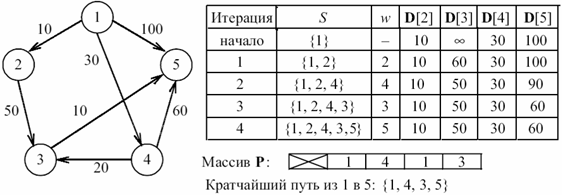
\includegraphics[width=13cm]{pic/45_01.png}

\end{figure}

\begin{lstlisting}[label=code:de,caption=Опис функції алгоритму Дейкстри]
  // Опис функції алгоритму Дейкстри
void Dijkstra (int n, int ** Graph, int Node) {
   bool * S = new bool [n];
   int * D = new int [n];
   int * P = new int [n];
   int i, j;
   int Max_Sum = 0;
   for (i = 0; i <n; i ++)
     for (j = 0; j <n; j ++)
       Max_Sum + = Graph [i] [j];
   for (i = 0; i <n; i ++)
     for (j = 0; j <n; j ++)
       if (Graph [i] [j] == 0) 
         Graph [i] [j] = Max_Sum;
   for (i = 0; i <n; i ++) {
     S [i] = false;
     P [i] = Node;
     D [i] = Graph [Node] [i];
   }
   S [Node] = true;
   P [Node] = -1;
   for (i = 0; i <n - 1; i ++) {
     int w = 0;
     for (j = 1; j <n; j ++) {
       if (! S [w]) {
         if (! S [j] && D [j] <= D [w])
           w = j;
       }
       else w ++;
     }
     S [w] = true;
     for (j = 1; j <n; j ++)
       if (! S [j])
         if (D [w] + Graph [w] [j] <D [j]) {
           D [j] = D [w] + Graph [w] [j];
           P [j] = w;
         }
   }
   for (i = 0; i <n; i ++)
     printf ("% 5d", D [i]);
   cout << endl;
   for (i = 0; i <n; i ++)
     printf ("% 5d", P [i] +1);
   cout << endl;
   delete [] P;
   delete [] D;
   delete [] S;
 } 
\end{lstlisting}

Складність алгоритму Дейкстри залежить від способу знаходження вершини, а також способу зберігання безлічі невідвіданих вершин і способи оновлення довжин.

Якщо для представлення графа використовувати матрицю суміжності, то час виконання цього алгоритму має порядок O (n 2), де n - кількість вершин графа. 

\subsection{Алгоритм Флойда}
Розглянутий алгоритм іноді називають алгоритмом Флойда -Уоршелла. Алгоритм Флойда -Уоршелла є алгоритмом на графах, який розроблений в 1962 році Робертом Флойдом і Стівеном Уоршеллом. Він служить для знаходження найкоротших шляхів між усіма парами вершин графа.

Метод Флойда безпосередньо грунтується на тому факті, що в графі з позитивними вагами ребер всякий Неелементарні (що містить більше 1 ребра) найкоротший шлях складається з інших найкоротших шляхів.

Цей алгоритм більш загальний порівняно з алгоритмом Дейкстри, оскільки він знаходить найкоротші шляхи між будь-якими двома вершинами графа.

В алгоритмі Флойда використовується матриця A розміром nxn, в якій обчислюються довжини найкоротших шляхів. Елемент A [i, j] дорівнює відстані від вершини i до вершини j, яке має кінцеве значення, якщо існує ребро (i, j), і дорівнює нескінченності в іншому випадку.

Алгоритм Флойда

Основна ідея алгоритму. Нехай є три вершини i, j, k і задані відстані між ними. Якщо виконується нерівність $A_{[i, k]} + A_{[k, j]} < A_{[i, j]}$, то доцільно замінити шлях i-> j шляхом i-> k-> j. Така заміна виконується систематично в процесі виконання даного алгоритму.

Крок 0. Визначаємо початкову матрицю відстані A 0 і матрицю послідовності вершин S 0. Кожен діагональний елемент обох матриць дорівнює 0, таким чином, показуючи, що ці елементи в обчисленнях не беруть участь. Вважаємо k = 1.

Основний крок k. Задаємо рядок k і стовпець k як провідну рядок і провідний стовпець. Розглядаємо можливість застосування заміни описаної вище, до всіх елементів A [i, j] матриці A k-1. Якщо виконується нерівність A [i, k] + A [k, j] <A [i, j], (i \ ne k, j \ ne k, i \ ne j) , Тоді виконуємо наступні дії:

    створюємо матрицю A k шляхом заміни в матриці A k-1 елемента A [i, j] на суму A [i, k] + A [k, j];
    створюємо матрицю S k шляхом заміни в матриці S k-1 елемента S [i, j] на k. Вважаємо k = k + 1 і повторюємо крок k. 

Таким чином, алгоритм Флойда робить n ітерацій, після i -й ітерації матриця А буде містити довжини найкоротших шляхів між будь-якими двома парами вершин за умови, що ці шляхи проходять через вершини від першої до i -й. На кожній ітерації перебираються всі пари вершин і шлях між ними скорочується за допомогою i -й вершини (рис.~\ref{pic:45.2}).
Демонстрація алгоритму Флойда
\begin{figure}
\caption{Демонстрація алгоритму Флойда}\label{pic:45.2}
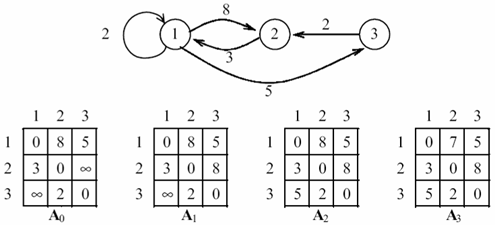
\includegraphics[width=13cm]{pic/45_02.png}

\end{figure}

\begin{lstlisting}[label=code:fl,caption=Опис функції алгоритму Флойда]
  // Опис функції алгоритму Флойда
 void Floyd (int n, int ** Graph, int ** ShortestPath) {
   int i, j, k;
   int Max_Sum = 0;
   for (i = 0; i <n; i ++)
     for (j = 0; j <n; j ++)
       Max_Sum + = ShortestPath [i] [j];
   for (i = 0; i <n; i ++)
     for (j = 0; j <n; j ++)
       if (ShortestPath [i] [j] == 0 && i! = j) 
         ShortestPath [i] [j] = Max_Sum;
   for (k = 0; k <n; k ++)
     for (i = 0; i <n; i ++)
       for (j = 0; j <n; j ++)
         if ((ShortestPath [i] [k] + ShortestPath [k] [j]) < 
              ShortestPath [i] [j])
           ShortestPath [i] [j] = ShortestPath [i] [k] + 
             ShortestPath [k] [j];
 } 
\end{lstlisting}
Зауважимо, що якщо граф неорієнтовний, то всі матриці, одержувані в результаті перетворень симетричні і, отже, досить вираховуватимуть тільки елементи, розташовані вище головної діагоналі.

Якщо граф представлений матрицею суміжності, то час виконання цього алгоритму має порядок O (n 3), оскільки в ньому присутні вкладені одна в одного три циклу. 


\subsection{Переборні алгоритми}

Переборні алгоритми по суті своїй є алгоритмами пошуку, як правило, пошуку оптимального рішення. При цьому рішення конструюється поступово. У цьому випадку зазвичай говорять про перебір вершин дерева варіантів. Вершинами такого графа будуть проміжні або кінцеві варіанти, а ребра вказуватимуть шляху конструювання варіантів.

Розглянемо Переборні алгоритми, засновані на методах пошуку в графі, на прикладі задачі знаходження найкоротшого шляху в лабіринті.

Постановка завдання.

Лабіринт, що складається з прохідних і непрохідних клітин, заданий матрицею A розміром mxn. Елемент матриці A [i, j] = 0, якщо клітина (i, j) прохідна. В іншому випадку $A_{[i, j]} = \infty $.

Потрібно знайти довжину найкоротшого шляху з клітини (1, 1) в клітину (m, n).

Фактично дана матриця суміжності (тільки в ній нулі замінені нескінченності, а одиниці - нулями). Лабіринт являє собою граф.

Вершинами дерева варіантів в даній задачі є шляхи, що починаються в клітці (1, 1). Ребра - показують хід конструювання цих шляхів і з'єднують два шляхи довжини k і k + 1, де другий шлях виходить з першого додаванням до шляху ще одного ходу.

Перебір з поверненням

Даний метод заснований на методі пошуку в глибину. Перебір з поверненням вважають методом проб і помилок ("спробуємо сходити в цю сторону: не вийде - повернемося і спробуємо в іншу"). Так як перебір варіантів здійснюється методом пошуку в глибину, то доцільно під час роботи алгоритму зберігати поточний шлях в дереві. Цей шлях являє собою стек Way.

Також необхідний масив Dist, розмірність якого відповідає кількості вершин графа, який зберігає для кожної вершини відстань від неї до вихідної вершини.

Нехай поточної є деяка клітина (на початку роботи алгоритму - клітина (1, 1)). Якщо для поточної клітини є клітина-сусід Neighbor, відсутня в Way, в яку на цьому шляху ще не ходили, то додаємо Neighbor в Way і поточної клітці присвоюємо Neighbor, інакше витягти з Way.

Наведене вище опис дає чітко зрозуміти, чому цей метод називається перебором з поверненням. Поверненню тут відповідає операція "витягти з Way", яка зменшує довжину Way на 1.

Перебір закінчується, коли Way порожній і робиться спроба повернення назад. У цій ситуації повертатися вже нікуди (рис.~\ref{pic:45.3}).

Way є поточним шляхом, але в процесі роботи необхідно зберігати і оптимальний шлях OptimalWay.

Удосконалення алгоритму можна зробити наступним чином: не дозволяти, щоб довжина Way була більше або дорівнює довжині OptimalWay. У цьому випадку, якщо і буде знайдений якийсь варіант, він свідомо не буде оптимальним. Таке удосконалення в загальному випадку означає, що як тільки поточний шлях стане свідомо неоптимальним, треба повернутися назад. Дане поліпшення алгоритму дозволяє в багатьох випадках сильно скоротити перебір.
Демонстрація алгоритму перебору з поверненням

\begin{figure}
\caption{Демонстрація алгоритму перебору з поверненням}\label{pic:45.3}
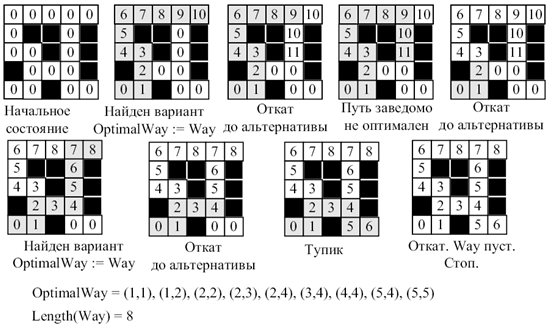
\includegraphics[width=13cm]{pic/45_03.png}
\end{figure}
\begin{lstlisting}
[label=code:pe,caption=Опис функції переборного алгоритму методом пошуку в глибину]
 / * Опис функції переборного алгоритму методом пошуку в глибину * /
void Backtracking (int n, int m, int ** Maze) {
  int Begin, End, Current;
  Begin = (n - 1) * m;
  End = m - 1;
  int * Way, * OptimalWay;
  int LengthWay, LengthOptimalWay;
  Way = new int [n * m];
  OptimalWay = new int [n * m];
  LengthWay = 0;
  LengthOptimalWay = m * n;
  for (int i = 0; i <n * m; i ++)
    Way [i] = OptimalWay [i] = -1;
  int * Dist;
  Dist = new int [n * m];
  for (int i = 0; i <n; i ++)
    for (int j = 0; j <m; j ++)
      Dist [i * m + j] = (Maze [i] [j] == 0? 0: -1);
  Way [LengthWay ++] = Current = Begin;
  while (LengthWay> 0) {
    if (Current == End) {
      if (LengthWay <LengthOptimalWay) {
        for (int i = 0; i <LengthWay; i ++)
          OptimalWay [i] = Way [i];
        LengthOptimalWay = LengthWay;
       }
      if (LengthWay> 0) Way [- LengthWay] = -1;
      Current = Way [LengthWay-1];
     }
    else {
      int Neighbor = -1;
      if ((Current / m - 1)> = 0 &&! Insert (Way, Current - m) &&
        (Dist [Current - m] == 0 || Dist [Current - m]> LengthWay)
        && Dist [Current] <LengthOptimalWay)
          Neighbor = Current - m;
       else 
        if ((Current% m - 1)> = 0 &&! Insert (Way, Current - 1) &&
          (Dist [Current - 1] == 0 || Dist [Current - 1]> LengthWay)
          && Dist [Current] <LengthOptimalWay)
            Neighbor = Current - 1;
         else 
          if ((Current% m + 1) <m &&! Insert (Way, Current + 1) &&
           (Dist [Current + 1] == 0 || Dist [Current + 1]> LengthWay)
          && Dist [Current] <LengthOptimalWay)
            Neighbor = Current + 1;
          else 
           if ((Current / m + 1) <n &&! Insert (Way, Current + m) &&
            (Dist [Current + m] == 0 || Dist [Current + m]> LengthWay)
           && Dist [Current] <LengthOptimalWay)
             Neighbor = Current + m;
      if (Neighbor! = -1) {
        Way [LengthWay ++] = Neighbor;
        Dist [Neighbor] = Dist [Current] + 1;
        Current = Neighbor;
       }
       else {
        if (LengthWay> 0) Way [- LengthWay] = -1;
        Current = Way [LengthWay-1];
       }
     }
   }
  if (LengthOptimalWay <n * m) 
    cout << endl << "Yes. Length way =" << LengthOptimalWay << endl;
  else cout << endl << "No" << endl;
 } 
\end{lstlisting}


\subsection{Хвильовий алгоритм}

Цей переборний алгоритм, який заснований на пошуку в ширину, складається з двох етапів:
\begin{itemize}
\item поширення хвилі;
\item зворотний хід.
\end{itemize}
 
Поширення хвилі і є власне пошук в ширину, при якому клітини позначаються номером кроку методу, на якому клітина відвідується. При зворотному ході, починаючи з кінцевої вершини, йде відновлення шляху, по якому в неї потрапили шляхом включення до нього клітин з мінімальною позначкою (рис.~\ref{pic:45.4}). Важливою особливістю є те, що відновлення починається з кінця (з початку воно найчастіше неможливо).
Демонстрація хвильового алгоритму

\begin{figure}
\caption{Демонстрація хвильового алгоритму}\label{pic:45.4}
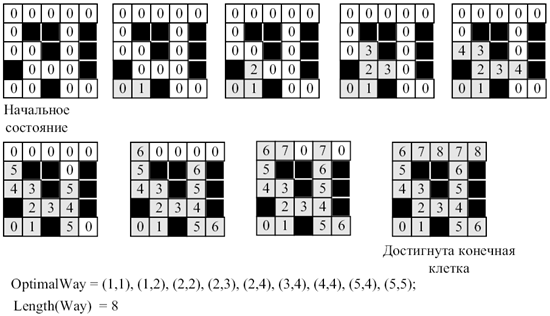
\includegraphics[width=13cm]{pic/45_04.png}
\end{figure}


Зауважимо, що перебір методом пошуку в ширину в порівнянні з перебором з поверненням, як правило, вимагає більше допоміжної пам'яті, яка необхідна для зберігання інформації, щоб побудувати шлях при зворотному ході і помітити відвідані вершини. Однак він працює швидше, оскільки абсолютно виключається відвідування однієї і тієї ж клітини більш ніж один раз.

\section{Приклади обчислень}
\nopagebreak[4]




\subsection*{Контрольні запитання}
\nopagebreak[4]
\begin{enumerate}
\item ?
\end{enumerate}




%\chapter{Використання багаторозгалужених дерев}
\nopagebreak[4]
\section*{Мета роботи}

\nopagebreak[4]
\section{Вступ}
\nopagebreak[4]


\section{Ключові терміни}
\nopagebreak[4]




\section{Розширені теоретичні відомості}
\nopagebreak[4]




\section{Приклади обчислень}
\nopagebreak[4]




\subsection*{Контрольні запитання}
\nopagebreak[4]
\begin{enumerate}
\item ?
\end{enumerate}




%\chapter{Алгоритми сортування}


\nopagebreak[4]
\section{Вступ}
\nopagebreak[4]
\textbf{Алгоритмом сортування} називається алгоритм для впорядкування деякого безлічі елементів. Зазвичай під алгоритмом сортування подразумевают алгоритм упорядкування безлічі елементів за зростанням або спаданням.

У разі наявності елементів з однаковими значеннями, у впорядкованій послідовності вони розташовуються поруч один за одним у будь-якому порядку. Однак іноді буває корисно зберігати первісний порядок елементів з однаковими значеннями.

Алгоритми сортування мають велике практичне застосування. Їх можна зустріти там, де мова йде про обробку та зберіганні великих обсягів інформації. Деякі завдання обробки даних вирішуються простіше, якщо дані заздалегідь впорядкувати.

\section{Ключові терміни}
\nopagebreak[4]




\section{Розширені теоретичні відомості}
\nopagebreak[4]
В алгоритмах сортування лише частина даних використовується як ключ сортування. Ключем сортування називається атрибут (або декілька атрибутів), за значенням якого визначається порядок елементів. Таким чином, при написанні алгоритмів сортувань масивів слід врахувати, що ключ повністю або частково збігається з даними.

Практично кожен алгоритм сортування можна розбити на 3 частини:
\begin{enumerate}
\item порівняння, визначальне впорядкованість пари елементів;
\item перестановку, змінюють місце пару елементів;
\item власне сортують алгоритм, який здійснює порівняння і перестановку елементів до тих пір, поки всі елементи множини не будуть впорядковані.
\end{enumerate}

\subsection{Оцінка алгоритмів сортування}

Жодна інша проблема не породила такої кількості найрізноманітніших рішень, як завдання сортування. Універсального, найкращого алгоритму сортування на даний момент не існує. Проте, маючи приблизні характеристики вхідних даних, можна підібрати метод, який працює оптимальним чином. Для цього необхідно знати параметри, за якими буде проводитися оцінка алгоритмів.

\textbf{Час сортування} - основний параметр, що характеризує швидкодію алгоритму.

\textbf{Пам'ять} - один з параметрів, який характеризується тим, що ряд алгоритмів сортування вимагають виділення додаткової пам'яті під тимчасове зберігання даних. При оцінці використовуваної пам'яті не враховуватиметься місце, яке займає вихідний масив даних і незалежні від вхідної послідовності витрати, наприклад, на зберігання коду програми.

\textbf{Стійкість} - це параметр, який відповідає за те, що сортування не змінює взаємного розташування рівних елементів.

\textbf{Природність поведінки} - параметр, якій вказує на ефективність методу при обробці вже відсортованих, або частково відсортованих даних. Алгоритм поводиться природно, якщо враховує цю характеристику вхідної послідовності і працює краще.

\subsection{Класифікація алгоритмів сортувань}

Все розмаїття і різноманіття алгоритмів сортувань можна класифікувати за різними ознаками, наприклад, по стійкості, по поведінці, по використанню операцій порівняння, за потреби в додатковій пам'яті, по потреби в знаннях про структуру даних, що виходять за рамки операції порівняння, та інші.

Найбільш докладно розглянемо класифікацію алгоритмів сортування за сферою застосування. У даному випадку основні типи впорядкування діляться наступним чином.

\textbf{Внутрішнє сортування} - це алгоритм сортування, який в процесі упорядкування даних використовує тільки оперативну пам'ять (ОЗП) на комп'ютері. Тобто оперативної пам'яті достатньо для завантаження в неї сортованого масиву даних з довільним доступом до будь-якій комірці і власне для виконання алгоритму. Внутрішня сортування застосовується у всіх випадках, за винятком однопрохідного зчитування даних і однопрохідної записи відсортованих даних. Залежно від конкретного алгоритму та його реалізації дані можуть сортуватися в тій же області пам'яті, або використовувати додаткову оперативну пам'ять.

\textbf{Зовнішнє сортування} - це алгоритм сортування, який при проведенні упорядкування даних використовує зовнішню пам'ять, як правило, жорсткі диски. Зовнішня сортування розроблена для обробки великих списків даних, які не поміщаються в оперативну пам'ять. Звернення до різних носіям накладає деякі додаткові обмеження на даний алгоритм: доступ до носія здійснюється послідовним чином, тобто в кожен момент часу можна вважати або записати тільки елемент, наступний за поточним; обсяг даних не дозволяє їм розміститися в ОЗУ.

Внутрішнє сортування є базовою для будь-якого алгоритму зовнішньої сортування - окремі частини масиву даних сортуються в оперативної пам'яті і за допомогою спеціального алгоритму зчіплюються в один масив, упорядкований по ключу.







%\chapter{Алгоритми внутрішнього сортування}
\nopagebreak[4]
\section*{Мета роботи}

\nopagebreak[4]
\section{Вступ}
\nopagebreak[4]


\section{Ключові терміни}
\nopagebreak[4]




\section{Розширені теоретичні відомості}
\nopagebreak[4]




\section{Приклади обчислень}
\nopagebreak[4]




\subsection*{Контрольні запитання}
\nopagebreak[4]
\begin{enumerate}
\item ?
\end{enumerate}




%\chapter{Алгоритми зовнішнього сортування}


\nopagebreak[4]
\section{Вступ}
\nopagebreak[4]
\textbf{Зовнішнє сортування} - сортування даних, розташованих на периферійних пристроях і не вміщаються в оперативну пам'ять, тобто коли застосувати одну з внутрішніх сортувань неможливо. Варто відзначити, що внутрішня сортування значно ефективніше зовнішньої, так як на звернення до оперативної пам'яті витрачається набагато менше часу, ніж до магнітних дисків, стрічок і т.п.

Найбільш часто зовнішнє сортування використовується в СУБД.

Дані, що зберігаються на зовнішніх пристроях, мають великий обсяг, що не дозволяє їх цілком перемістити в оперативну пам'ять, відсортувати з використанням одного з алгоритмів внутрішнього сортування, а потім повернути їх на зовнішній пристрій. У цьому випадку здійснювалося б мінімальну кількість проходів через файл, тобто було б однократне читання і однократна запис даних. Однак на практиці доводиться здійснювати читання, обробку і запис даних у файл по блоках, розмір яких залежить від операційної системи та наявного обсягу оперативної пам'яті, що призводить до збільшення числа проходів через файл і помітного зниження швидкості сортування.

\section{Ключові терміни}
\nopagebreak[4]
\textbf{Зовнішнє сортування} - це сортування даних, які розташовані на зовнішніх пристроях і не вміщаються в оперативну пам'ять.

\textbf{Фаза} - це дії по одноразовій обробці всієї послідовності елементів.

\textbf{Серія (упорядкований відрізок)} - це послідовність елементів, що упорядкована по ключу. Кількість елементів в серії називається довжиною серії.

\textbf{Двофазне сортування} - це сортування, в якому окремо реалізується дві фази: розподіл і злиття. 

\textbf{Однофазне сортування} - це сортування, в якому об'єднані фази розподілу і злиття в одну.

\textbf{Двоколійним злиттям} називається сортування, в якому дані розподіляються на два допоміжних файли. 

\textbf{Багатоколійним злиттям} називається сортування, в якому дані розподіляються на N (N> 2) допоміжних файлів.



\section{Розширені теоретичні відомості}
\nopagebreak[4]

\subsection{Сортування простим злиттям}

Одне з сортувань на основі злиття називається простим злиттям.

Алгоритм сортування простим злиття є найпростішим алгоритмом зовнішньої сортування, заснований на процедурі злиття серією.

У даному алгоритмі довжина серій фіксується на кожному кроці. У вихідному файлі всі серії мають довжину 1, після першого кроку вона дорівнює 2, після другого - 4, після третього - 8, після k-го кроку - 2k.

Алгоритм сортування простим злиттям

\begin{enumerate}
\item Вихідний файл f розбивається на два допоміжних файлу f1 і f2.

\item Допоміжні файли f1 і f2 зливаються в файл f, при цьому поодинокі елементи утворюють впорядковані пари.

\item Отриманий файл f знову обробляється, як зазначено в кроках 1 і 2. При цьому впорядковані пари переходять у впорядковані четвірки.

\item Повторюючи кроки, зливаємо четвірки в вісімки і т.д., кожен раз подвоюючи довжину злитих послідовностей до тих пір, поки не буде впорядкований цілком весь файл (рис.~\ref{f:sort1}).
\end{enumerate}

\begin{figure}
\caption{Демонстрація сортування двоколійному двофазним простим злиттям}\label{f:sort1}
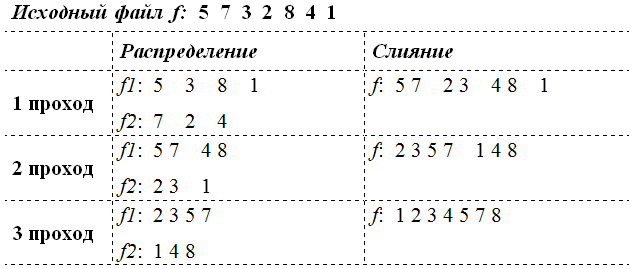
\includegraphics[width=13cm]{pic/43_01.png}

\end{figure}

Після виконання i проходів отримуємо два файли, що складаються з серій довжини 2i. Закінчення процесу відбувається при виконанні умови $2^i \geq n$. Отже, процес сортування простим злиттям вимагає порядку $O (\log n)$ проходів за даними.

Ознаками кінця сортування простим злиттям є наступні умови:

\begin{enumerate}
\item довжина серії не менша кількість елементів у файлі (визначається після фази злиття);
\item кількість серій рівно 1 (визначається на фазі злиття).
\item при однофазному сортуванні другий за рахунком допоміжний файл після розподілу серій залишився порожнім.
\end{enumerate}

Приклад програмної реалізації надано у додатку \ref{code:sort111};

\section{Приклади обчислень}
\nopagebreak[4]







%\chapter{Характеристика алгоритмів порівняння методів сортування}
\nopagebreak[4]
\section*{Мета роботи}

\nopagebreak[4]
\section{Вступ}
\nopagebreak[4]


\section{Ключові терміни}
\nopagebreak[4]




\section{Розширені теоретичні відомості}
\nopagebreak[4]




\section{Приклади обчислень}
\nopagebreak[4]




\subsection*{Контрольні запитання}
\nopagebreak[4]
\begin{enumerate}
\item ?
\end{enumerate}




\appendix
\makeatletter
\gdef\thechapter{\@Asbuk\c@chapter}
\makeatother
\def\chaptername{Додаток}


\chapter{Правила оформлення звіту}
\section{Титульна сторінка лабораторної роботи}
%\begin{titlepage}
%\newpage

\hrulefill

\begin{center}
МІНІСТЕРСТВО ОСВІТИ І НАУКИ, МОЛОДІ ТА СПОРТУ УКРАЇНИ \\

ХЕРСОНСЬКИЙ НАЦІОНАЛЬНИЙ ТЕХНІЧНИЙ УНІВЕРСИТЕТ \\*

КАФЕДРА ІНФОРМАЦІЙНИХ ТЕХНОЛОГІЙ

\end{center}

\vspace{5em}

\begin{center}
\Large Звіт до лабораторної роботи \No 123 \\ з дисципліни <<Web-програмування>>
\end{center}

\vspace{2.5em}

\begin{center}
{\Large Тема: \textbf{<<Основи мережі Internet>>}}
\end{center}

\vspace{5em}





\begin{flushleft}
Виконав \\ст.групи хПР1 \hspace{\fill} Пупкін А.А. \\
\vspace{1em}
Перевірив \\ст.викладач \hspace{\fill} Іванов Б.Б.\\
\end{flushleft}

\vspace{\fill}

\begin{center}
Херсон 2012
\end{center}
\newpage
%\end{titlepage}
\section{Приклади блок-схем}
Правила виконання блок-схем задані наступними документами:
\begin{itemize}
\item ГОСТ 19.701-90. Схемы алгоритмов, программ, данных и систем. Условные обозначения и правила выполнения
\item ГОСТ 19.002-80. Схемы алгоритмов и программ. Правила выполнения
\item ГОСТ 19.003-80. Схемы алгоритмов и программ. Обозначения условные графические

\end{itemize}



%\include{ap02}
%\include{ap03}
%\include{ap04}
%\include{ap05}
%\include{ap06}
%\include{ap07}
%\include{ap08}
%\include{ap09}
%\include{ap10}
 
 



%% указываем класс документа
%\documentclass[twoside,8pt,a5paper,openany]{report}
\documentclass[twoside,12pt,a4paper,openany]{report}

% подключаем собственный стилевой файл
\usepackage{labstyle}
\usepackage{labstyle2}







\makeindex





\begin{document}


% указываем язык (для автоматической вставки слов, типа "Глава", "Содержание", "Литература", "рис." и пр.
\selectlanguage{ukrainian}



% подключаем файлы содержимого
\begin{titlepage}
\newpage

\begin{center}
МІНІСТЕРСТВО ОСВІТИ І НАУКИ УКРАЇНИ \\

ХЕРСОНСЬКИЙ ПОЛІТЕХНІЧНИЙ КОЛЕДЖ \\

ОДЕСЬКОГО НАЦІОНАЛЬНОГО ПОЛІТЕХНІЧНОГО УНІВЕРСИТЕТУ\\

ВІДДІЛЕННЯ КОМП'ЮТЕРНОЇ ТА ПРОГРАМНОЇ ІНЖЕНЕРІЇ

\end{center}


\vspace{10em}

\begin{center}
\Large Курс лекції \\ з дисципліни
\end{center}

\vspace{2em}

\begin{center}
\huge{\textbf{<<Алгоритми та структури даних>>}}
\end{center}




\vspace{\fill}

\begin{center}
Херсон --- 2015
\end{center}

\end{titlepage}



% ненужное можно просто закомментировать знаком процента "%" 

% первую страницу не нумеруем
%\thispagestyle{empty}			

% название
%\title{Методичні вказівки до лабораторних робіт з дисципліни <<web-програмування>>}
%\author{Жарікова М.В., Левицький В.М.}
%\maketitle

% печатаем содержание
%\chapter*[Зміст]{Зміст}
\tableofcontents

% ничанаем с новой страницы
%\newpage

% печатаем перечень рисунков
%\chapter*{Перелік ілюстрацій}
\listoffigures

% печатаем перечень таблиц
%\chapter*{Перелік таблиць}
\listoftables

\lstlistoflistings

%\lstlistoflistings


\chapter{Рекурсія і рекурсивні алгоритми}
\nopagebreak[4]
\section*{Мета роботи}
Вивчити поняття, види рекурсії і рекурсивну тріаду, навчитися розробляти рекурсивну тріаду при вирішенні завдань мовою C++.

При виконанні лабораторної роботи для кожного завдання потрібно написати програму на мові С++, яка отримує на вході числові дані, виконує їх обробку відповідно до вимог завдання і виводить результат на екран. Для обробки даних необхідно реалізувати рекурсивну функцію. Введення даних здійснюється з клавіатури з урахуванням вимог до вхідних даних, що містяться в постановці завдання (введення даних супроводжуйте діалогом). Обмеженнями на вхідні дані є допустимий діапазон значень використовуваних числових типів в мові С++.

\nopagebreak[4]
\section{Теоретичнi вiдомостi}

\begin{lstlisting}[label=code:rec1,caption=Програма обчислення факторіалу ітераційним способом]
public class App {
    public static void main(String[] args) {
        System.out.println(factorial(5));
    }
     
    public static int factorial(int arg) {
        int result = 1;
        for (int k = 1; k <= arg; k++) {
            result *= k;
        }
        return result;
    }
}
 
>> 120
\end{lstlisting}

\begin{lstlisting}[label=code:rec1,caption=Програма обчислення факторіалу рекурсивним способом]
public class App {
    public static void main(String[] args) {
        System.out.println(factorial(5));
    }
     
    public static int factorial(int arg) {
        if (arg == 1) {
            return 1;
        } else {
            return arg * factorial(arg - 1);
        }
    }
}
 
>> 120
\end{lstlisting}
\nopagebreak[4]
\section{Вказівки до виконання роботи.}
\nopagebreak[4]

Кожне завдання необхідно вирішити вивченими рекурсивними методами вирішення завдань і методами обробки числових даних у мові С++. Перед реалізацією коду кожного завдання необхідно розробити рекурсивну тріаду відповідно до постановкою завдання: виконати параметризацію, виділити базу і оформити декомпозицію рекурсії. Програму для вирішення кожного завдання необхідно розробити методом процедурної абстракції, використовуючи рекурсивні функції. Етапи супроводити коментарями в коді.

Слід реалізувати кожне завдання у відповідності з наведеними етапами:

\begin{itemize}
\item вивчити словесну постановку задачі, виділивши при цьому всі види даних;
\item сформулювати математичну постановку задачі;
\item вибрати метод розв'язання задачі, якщо це необхідно;
\item розробити графічну схему алгоритму;
\item записати розроблений алгоритм на мові С ++;
\item розробити контрольний тест до програми;
\item налагодити програму;
\item подати звіт по роботі. 
\end{itemize}



\section{Індивідуальне завдання}
\nopagebreak[4]
\subsection*{Завдання до лабораторної роботи}
\nopagebreak[4]
\begin{enumerate}
\item Створіть програму для обчислення $n$-го числі Фібоначчі.

\end{enumerate}

\subsection*{Контрольні запитання}
\nopagebreak[4]
\begin{enumerate}
\item Чи можна випадок непрямої рекурсії звести до прямої рекурсії? Відповідь обґрунтуйте.
\item Чи може рекурсивна база містити кілька тривіальних випадків? Відповідь обґрунтуйте.
\item Чи є параметри, база і декомпозиція єдиними для конкретного завдання? Відповідь обґрунтуйте.
\item З якою метою в задачах відбувається перегляд або коригування обраних параметрів, виділеної бази або випадку декомпозиції?
\item Чи є рекурсія універсальним способом вирішення завдань? Відповідь обґрунтуйте.
\item Чому для оцінки трудомісткості рекурсивного алгоритму недостатньо одного методу підрахунку вершин рекурсивного дерева?


\end{enumerate}




\chapter{Рекурсія}
\nopagebreak[4]
\section*{Мета роботи}

\nopagebreak[4]
\section{Вступ}
\nopagebreak[4]
У математиці для вирішення переважної більшості завдань використовуються методи, які в кінцевому рахунку можуть бути зведені до одного з двох базових способів: ітерації або рекурсії.


\textbf{Ітерація} означає кількаразове повторення одних і тих же дій, яке після деякої кількості кроків приводить до бажаного результату. Характерним прикладом ітераційного способу вирішення завдання є методи послідовних наближень рішення нелінійних рівнянь, у тому числі метод дотичних, метод хорд і т.д.

\begin{equation}
f(x)=0; x=\varphi(x); x_0=a; x_n=\varphi(x_{n-1}), n=1,2,..., |x_k-x_{k-1}|>\epsilon
\end{equation}

\textbf{Рекурсія} являє собою посилання при описі об'єкта, дії на описуваний об'єкт, дія. Рекурсія означає рішення задачі за допомогою відомості рішення до самого себе. При цьому обчислення залежать від інших, в не-якому сенсі більш простих (зазвичай менших) значень аргументу або аргументів завдання. Повністю аналогічні механізми використовуються в базовій теорії рекурсивних функцій, у методі математичної індукції, а також в рекурентних послідовностях. 

Наприклад:

\begin{equation}
a_k = 2a_{k-1} + k , \forall k > 0, a_0 = 1
\end{equation}

\textbf{Рекурсивний алгоритм} - це алгоритм, в описі якого прямо або побічно міститься звернення до самого себе. У техніці процедурного програмування дане поняття поширюється на функцію, яка реалізує рішення окремого блоку завдання за допомогою виклику зі свого тіла інших функцій, в тому числі і себе самої. Якщо при цьому на черговому етапі роботи функція організовує звернення до самої себе, то така функція є рекурсивної.



\section{Ключові терміни}
\nopagebreak[4]


\textbf{База рекурсії} - це тривіальний випадок, при якому рішення задачі очевидно, тобто не потрібно звернення функції до себе.

\textbf{Глибина рекурсивних викликів} - це найбільше одночасне кількість рекурсивних звернень функції, визначальне максимальну кількість шарів рекурсивного стека.

\textbf{Декомпозиція} - це вираження загального випадку через більш прості підзадачі зі зміненими параметрами.

\textbf{Корінь повного дерева рекурсивних викликів} - це вершина повного дерева рекурсії, відповідна початкового зверненням до функції.

\textbf{Непряма (взаємна) рекурсія} - це послідовність взаємних викликів декількох функцій, організована у вигляді циклічного замикання на тіло первісної функції, але з іншим набором параметрів.

\textbf{Обсяг рекурсії} - це характеристика складності рекурсивних обчислень для конкретного набору параметрів, що представляє собою кількість вершин повного рекурсивного дерева без одиниці.

\textbf{Параметризація} - це виділення з постановки задачі параметрів, які використовуються для опису умови задачі і рішення.

\textbf{Повне дерево рекурсії} - це граф, вершинами якого є набори фактичних параметрів при всіх викликах функції, починаючи з першого звернення до неї, а ребрами - пари таких наборів, відповідних взаємним викликам.

\textbf{Пряма рекурсія} - це безпосереднє звернення рекурсивної функції до себе, але з іншим набором вхідних даних.

\textbf{Рекурсивна тріада} - це етапи вирішення завдань рекурсивним методом.

\textbf{Рекурсивна функція} - це функція, яка у своєму тілі містить звернення до самої себе зі зміненим набором параметрів.

\textbf{Рекурсивний алгоритм} - це алгоритм, у визначенні якого міститься прямий або непрямий виклик цього ж алгоритму.

\textbf{Рекурсія} - це визначення об'єкта за допомогою посилання на себе.


\section{Розширені теоретичні відомості}
\nopagebreak[4]


Рекурсивні алгоритми зазвичай виходять на основі математичної постановки завдання. Найважливіше при побудові рекурсивного алгоритму: побачити однакові дії на поточному та попередньому кроці обчислень (дій).

Виконавець рекурсивного алгоритму зводить невідоме до іншого невідомого, накопичуючи інформацію (прямий хід) і відкладаючи фактичні обчислення до моменту, коли виконається умова, що дозволяють безпосередньо обчислити шукане значення. Потім виконується зворотний хід рекурсії.

\textbf{Основні переваги рекурсії:}
\begin{itemize}
\item простота математичного формулювання;
\item простота алгоритму і його реалізації
\end{itemize}
\textbf{Основні недоліки рекурсії:}
\begin{itemize}
\item додаткові витрати оперативної пам'яті;
\item додаткові тимчасові витрати;
\item можливий перехід складності в клас EXP.
\end{itemize}

За аналогією з математичної індукцією, на яку рекурсія трохи схожа, будь рекурсивна процедура повинна включати в себе базис і крок рекурсії.

Базис рекурсії - це пропозиція, що визначає якусь початкову ситуацію або ситуацію в момент припинення. Як правило, в цій пропозиції записується якийсь найпростіший випадок, при якому відповідь виходить відразу навіть без використання рекурсії. Так, у наведеній вище процедурі, яка описує предикат предок, базисом рекурсії є перше правило, в якому визначено, що найближчими предками людини є його батьки. Ця пропозиція часто містить умову, при виконанні якї відбувається вихід з рекурсії або відсікання.

Крок рекурсії - це правило, в тілі якого обов'язково міститься, в якості підцілі, виклик обумовленого предиката. Якщо ми хочемо уникнути зациклення, який визначається предикат повинен викликатися не вiд тих же параметрів, які вказані в заголовку правила. Параметри повинні змінюватися на кожному кроці так, щоб в результаті або спрацював базис рекурсії, або умова виходу з рекурсії, розміщене в самому правилі.

\section{Приклади обчислень}
\nopagebreak[4]


\subsection*{Приклад 1. Обчислення факторіала $P=n!$, n - ціле число}

Зазвичай для обчислення факторіала цілого числа використовується ітераційний спосіб, заснований на багаторазовому домноженні величини, в якій накопичується результат, на черговий співмножник: 

\begin{equation}
Pi := P_{i-1} \times i, i=2,3,...,k.  
\end{equation}

\begin{lstlisting}[label=iter1,caption=Ітераційна функція] 
function factorial (k:integer):integer;
	var P,i:integer;  { i – номер сомножителя, P – накапливаемый результат}
begin
	P:=1;
	for i:=1 to k do
		P:=P*i;
	factorial:=P;
end;
\end{lstlisting}

Це завдання можна вирішити і за допомогою рекурсії, базуючись на наступних міркуваннях:

\begin{equation}
k! = 1 \times 2 \times 3 \times \dots \times k =  1 \times 2 \times 3 \times \dots \times (k-1) \times k = (k-1)! \times k
\end{equation}

Отже, $P(k) = k!$ можна визначити таким чином:

\begin{equation}
P(k) = 
 \begin{cases}
   1,k=1\\
   P(k-1)\times k,k>1
 \end{cases}
\end{equation}

\begin{lstlisting}[label=iter1,caption=Рекурентна функція] 
function factorial1 (k:integer):integer ;
begin
	if k=1 then factorial1:=1 
		else  factorial1:= factorial1(k-1)*k
end;
\end{lstlisting}




\section{Індивідуальне завдання}
\nopagebreak[4]
\subsection*{Завдання до лабораторної роботи}
\nopagebreak[4]
\begin{enumerate}
\item Вивчити теоретичний матеріал
\item Відповісти на контрольні запитання
\item Скласти звіт
\item Захистити роботу
\end{enumerate}

\subsection*{Контрольні запитання}
\nopagebreak[4]
\begin{enumerate}
\item Що таке Internet? З яких структурних частин складається Internet?
\item Що таке IP-адреса?
\item Що таке доменне ім'я, з чого воно складається?
\item Який сервіс Internet перетворює IP-адреси в доменні імена і навпаки?
\item Яка служба займається розподіленням блоків IP-адрес?
\item Протокол HTTP. Рівень у моделі OSI, призначення.
\item Значення URI, URL, URN.
\item Мови web-програмування, які ви знаєте.
\item Веб-сервери, які ви знаєте.
\item Мережеві СКБД, які ви знаєте. 
\end{enumerate}




\chapter{Представлення виразів за допомогою дерев}
\nopagebreak[4]
\section*{Мета роботи}

\nopagebreak[4]
\section{Вступ}
\nopagebreak[4]


\section{Ключові терміни}
\nopagebreak[4]




\section{Розширені теоретичні відомості}
\nopagebreak[4]




\section{Приклади обчислень}
\nopagebreak[4]




\subsection*{Контрольні запитання}
\nopagebreak[4]
\begin{enumerate}
\item ?
\end{enumerate}
%\chapter{Представлення багаторозгалужених дерев}
\nopagebreak[4]
\section*{Мета роботи}

\nopagebreak[4]
\section{Вступ}
\nopagebreak[4]


\section{Ключові терміни}
\nopagebreak[4]




\section{Розширені теоретичні відомості}
\nopagebreak[4]




\section{Приклади обчислень}
\nopagebreak[4]




\subsection*{Контрольні запитання}
\nopagebreak[4]
\begin{enumerate}
\item ?
\end{enumerate}




%\chapter{Представлення графів}
\nopagebreak[4]
\section*{Мета роботи}

\nopagebreak[4]
\section{Вступ}
\nopagebreak[4]


\section{Ключові терміни}
\nopagebreak[4]




\section{Розширені теоретичні відомості}
\nopagebreak[4]




\section{Приклади обчислень}
\nopagebreak[4]




\subsection*{Контрольні запитання}
\nopagebreak[4]
\begin{enumerate}
\item ?
\end{enumerate}



 
%\chapter{Алгоритми на графах}
\nopagebreak[4]

\section{Вступ}
\nopagebreak[4]
Знаходження найкоротшого шляху на сьогоднішній день є життєво необхідним завданням і використовується практично скрізь, починаючи від знаходження оптимального маршруту між двома об'єктами на місцевості (наприклад, найкоротший шлях від будинку до університету), в системах автопілота, для знаходження оптимального маршруту при перевезеннях, комутації інформаційного пакету в мережах і т.п.

Найкоротший шлях розглядається за допомогою деякого математичного об'єкта, званого графом. Пошук найкоротшого шляху ведеться між двома заданими вершинами в графі. Результатом є шлях, тобто послідовність вершин і ребер, інцидентних двом сусіднім вершинам, і його довжина.

Розглянемо три найбільш ефективних алгоритму знаходження найкоротшого шляху:

\begin{itemize}
\item алгоритм Дейкстри;
\item алгоритм Флойда;
\item Переборні алгоритми. 
\end{itemize}

Зазначені алгоритми легко виконуються при малій кількості вершин у графі. При збільшенні їх кількості завдання пошуку найкоротшого шляху ускладнюється. 




\section{Ключові терміни}
\nopagebreak[4]
\textbf{Алгоритм Дейкстри} - це алгоритм знаходження найкоротшого шляху від однієї з вершин графа до всіх інших, який працює тільки для графів без ребер негативного ваги.

\textbf{Алгоритм Флойда} - це алгоритм пошуку найкоротшого шляху між будь-якими двома вершинами графа.

\textbf{Хвильовий алгоритм} - це переборний алгоритм, який заснований на пошуку в ширину і складається з двох етапів: поширення хвилі і зворотний хід.

\textbf{Найкоротший шлях} - це шлях в графі, тобто послідовність вершин і ребер, інцидентних двом сусіднім вершинам, і його довжина.

Переборний алгоритм - це алгоритм обходу графа, заснований на послідовному переборі можливих шляхів.



\section{Розширені теоретичні відомості}
\subsection{Алгоритм Дейкстри}
\nopagebreak[4]

Даний алгоритм є алгоритмом на графах, який винайдений нідерландським вченим Е. Дейкстрой в 1959 році. Алгоритм знаходить найкоротший відстань від однієї з вершин графа до всіх інших і працює тільки для графів без ребер негативного ваги.

Кожній вершині приписується вага - це вага шляху від початкової вершини до даної. Також кожна вершина може бути виділена. Якщо вершина виділена, то шлях від неї до початкової вершини найкоротший, якщо ні - то тимчасовий. Обходячи граф, алгоритм вважає для кожної вершини маршрут, і, якщо він виявляється найкоротшим, виділяє вершину. Вагою даної вершини стає вага шляху. Для всіх сусідів даної вершини алгоритм також розраховує вагу, при цьому ні за яких умов не виділяючи їх. Алгоритм закінчує свою роботу, дійшовши до кінцевої вершини, і вагою найкоротшого шляху стає вага кінцевої вершини.

Алгоритм Дейкстри
\begin{enumerate}
\item Всім вершинам, за винятком першої, присвоюється вага рівний нескінченності, а першій вершині - 0.

\item Всі вершини не виділені.

\item Перша вершина оголошується поточної.

\item Вага всіх невиділених вершин перераховується за формулою: вага невиділеної вершини є мінімальне число зі старого ваги даної вершини, суми ваги поточної вершини і ваги ребра, що з'єднує поточну вершину з невиділеної.

\item Серед невиділених вершин шукається вершина з мінімальною вагою. Якщо така не знайдена, тобто вага всіх вершин дорівнює нескінченності, то маршрут не існує. Отже, вихід. Інакше, поточної стає знайдена вершина. Вона ж виділяється.

\item Якщо поточною вершиною виявляється кінцева, то шлях знайдений, і його вага є вага кінцевої вершини.

\item Перехід на крок 4.
\end{enumerate}

У програмній реалізації алгоритму Дейкстри побудуємо безліч S вершин, для яких найкоротші шляхи від початкової вершини вже відомі. На кожному кроці до множини S додається та з решти вершин, відстань до якої від початкової вершини менше, ніж для інших, що залишилися вершин. При цьому будемо використовувати масив D, в який записуються довжини найкоротших шляхів для кожної вершини. Коли безліч S буде містити всі вершини графа, тоді масив D міститиме довжини найкоротших шляхів від початкової вершини до кожної вершини.

Крім зазначених масивів будемо використовувати матрицю довжин C, де елемент C [i, j] - довжина ребра (i, j), якщо ребра немає, то її довжина покладається рівною нескінченності, тобто більше будь фактичної довжини ребер. Фактично матриця C являє собою матрицю суміжності, в якій всі нульові елементи замінені на нескінченність.

Для визначення самого найкоротшого шляху введемо масив P вершин, де P [v] буде містити вершину, безпосередньо попередню вершині v в найкоротшому шляху (рис.~\ref{pic:45.1}).
Демонстрація алгоритмом Дейкстри
\begin{figure}
\caption{Демонстрація алгоритму Дейкстри}\label{pic:45.1}
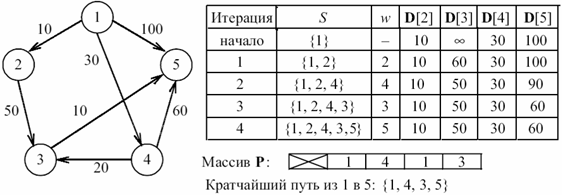
\includegraphics[width=13cm]{pic/45_01.png}

\end{figure}

\begin{lstlisting}[label=code:de,caption=Опис функції алгоритму Дейкстри]
  // Опис функції алгоритму Дейкстри
void Dijkstra (int n, int ** Graph, int Node) {
   bool * S = new bool [n];
   int * D = new int [n];
   int * P = new int [n];
   int i, j;
   int Max_Sum = 0;
   for (i = 0; i <n; i ++)
     for (j = 0; j <n; j ++)
       Max_Sum + = Graph [i] [j];
   for (i = 0; i <n; i ++)
     for (j = 0; j <n; j ++)
       if (Graph [i] [j] == 0) 
         Graph [i] [j] = Max_Sum;
   for (i = 0; i <n; i ++) {
     S [i] = false;
     P [i] = Node;
     D [i] = Graph [Node] [i];
   }
   S [Node] = true;
   P [Node] = -1;
   for (i = 0; i <n - 1; i ++) {
     int w = 0;
     for (j = 1; j <n; j ++) {
       if (! S [w]) {
         if (! S [j] && D [j] <= D [w])
           w = j;
       }
       else w ++;
     }
     S [w] = true;
     for (j = 1; j <n; j ++)
       if (! S [j])
         if (D [w] + Graph [w] [j] <D [j]) {
           D [j] = D [w] + Graph [w] [j];
           P [j] = w;
         }
   }
   for (i = 0; i <n; i ++)
     printf ("% 5d", D [i]);
   cout << endl;
   for (i = 0; i <n; i ++)
     printf ("% 5d", P [i] +1);
   cout << endl;
   delete [] P;
   delete [] D;
   delete [] S;
 } 
\end{lstlisting}

Складність алгоритму Дейкстри залежить від способу знаходження вершини, а також способу зберігання безлічі невідвіданих вершин і способи оновлення довжин.

Якщо для представлення графа використовувати матрицю суміжності, то час виконання цього алгоритму має порядок O (n 2), де n - кількість вершин графа. 

\subsection{Алгоритм Флойда}
Розглянутий алгоритм іноді називають алгоритмом Флойда -Уоршелла. Алгоритм Флойда -Уоршелла є алгоритмом на графах, який розроблений в 1962 році Робертом Флойдом і Стівеном Уоршеллом. Він служить для знаходження найкоротших шляхів між усіма парами вершин графа.

Метод Флойда безпосередньо грунтується на тому факті, що в графі з позитивними вагами ребер всякий Неелементарні (що містить більше 1 ребра) найкоротший шлях складається з інших найкоротших шляхів.

Цей алгоритм більш загальний порівняно з алгоритмом Дейкстри, оскільки він знаходить найкоротші шляхи між будь-якими двома вершинами графа.

В алгоритмі Флойда використовується матриця A розміром nxn, в якій обчислюються довжини найкоротших шляхів. Елемент A [i, j] дорівнює відстані від вершини i до вершини j, яке має кінцеве значення, якщо існує ребро (i, j), і дорівнює нескінченності в іншому випадку.

Алгоритм Флойда

Основна ідея алгоритму. Нехай є три вершини i, j, k і задані відстані між ними. Якщо виконується нерівність $A_{[i, k]} + A_{[k, j]} < A_{[i, j]}$, то доцільно замінити шлях i-> j шляхом i-> k-> j. Така заміна виконується систематично в процесі виконання даного алгоритму.

Крок 0. Визначаємо початкову матрицю відстані A 0 і матрицю послідовності вершин S 0. Кожен діагональний елемент обох матриць дорівнює 0, таким чином, показуючи, що ці елементи в обчисленнях не беруть участь. Вважаємо k = 1.

Основний крок k. Задаємо рядок k і стовпець k як провідну рядок і провідний стовпець. Розглядаємо можливість застосування заміни описаної вище, до всіх елементів A [i, j] матриці A k-1. Якщо виконується нерівність A [i, k] + A [k, j] <A [i, j], (i \ ne k, j \ ne k, i \ ne j) , Тоді виконуємо наступні дії:

    створюємо матрицю A k шляхом заміни в матриці A k-1 елемента A [i, j] на суму A [i, k] + A [k, j];
    створюємо матрицю S k шляхом заміни в матриці S k-1 елемента S [i, j] на k. Вважаємо k = k + 1 і повторюємо крок k. 

Таким чином, алгоритм Флойда робить n ітерацій, після i -й ітерації матриця А буде містити довжини найкоротших шляхів між будь-якими двома парами вершин за умови, що ці шляхи проходять через вершини від першої до i -й. На кожній ітерації перебираються всі пари вершин і шлях між ними скорочується за допомогою i -й вершини (рис.~\ref{pic:45.2}).
Демонстрація алгоритму Флойда
\begin{figure}
\caption{Демонстрація алгоритму Флойда}\label{pic:45.2}
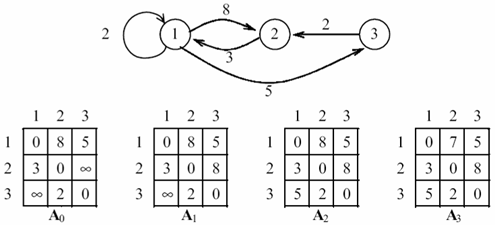
\includegraphics[width=13cm]{pic/45_02.png}

\end{figure}

\begin{lstlisting}[label=code:fl,caption=Опис функції алгоритму Флойда]
  // Опис функції алгоритму Флойда
 void Floyd (int n, int ** Graph, int ** ShortestPath) {
   int i, j, k;
   int Max_Sum = 0;
   for (i = 0; i <n; i ++)
     for (j = 0; j <n; j ++)
       Max_Sum + = ShortestPath [i] [j];
   for (i = 0; i <n; i ++)
     for (j = 0; j <n; j ++)
       if (ShortestPath [i] [j] == 0 && i! = j) 
         ShortestPath [i] [j] = Max_Sum;
   for (k = 0; k <n; k ++)
     for (i = 0; i <n; i ++)
       for (j = 0; j <n; j ++)
         if ((ShortestPath [i] [k] + ShortestPath [k] [j]) < 
              ShortestPath [i] [j])
           ShortestPath [i] [j] = ShortestPath [i] [k] + 
             ShortestPath [k] [j];
 } 
\end{lstlisting}
Зауважимо, що якщо граф неорієнтовний, то всі матриці, одержувані в результаті перетворень симетричні і, отже, досить вираховуватимуть тільки елементи, розташовані вище головної діагоналі.

Якщо граф представлений матрицею суміжності, то час виконання цього алгоритму має порядок O (n 3), оскільки в ньому присутні вкладені одна в одного три циклу. 


\subsection{Переборні алгоритми}

Переборні алгоритми по суті своїй є алгоритмами пошуку, як правило, пошуку оптимального рішення. При цьому рішення конструюється поступово. У цьому випадку зазвичай говорять про перебір вершин дерева варіантів. Вершинами такого графа будуть проміжні або кінцеві варіанти, а ребра вказуватимуть шляху конструювання варіантів.

Розглянемо Переборні алгоритми, засновані на методах пошуку в графі, на прикладі задачі знаходження найкоротшого шляху в лабіринті.

Постановка завдання.

Лабіринт, що складається з прохідних і непрохідних клітин, заданий матрицею A розміром mxn. Елемент матриці A [i, j] = 0, якщо клітина (i, j) прохідна. В іншому випадку $A_{[i, j]} = \infty $.

Потрібно знайти довжину найкоротшого шляху з клітини (1, 1) в клітину (m, n).

Фактично дана матриця суміжності (тільки в ній нулі замінені нескінченності, а одиниці - нулями). Лабіринт являє собою граф.

Вершинами дерева варіантів в даній задачі є шляхи, що починаються в клітці (1, 1). Ребра - показують хід конструювання цих шляхів і з'єднують два шляхи довжини k і k + 1, де другий шлях виходить з першого додаванням до шляху ще одного ходу.

Перебір з поверненням

Даний метод заснований на методі пошуку в глибину. Перебір з поверненням вважають методом проб і помилок ("спробуємо сходити в цю сторону: не вийде - повернемося і спробуємо в іншу"). Так як перебір варіантів здійснюється методом пошуку в глибину, то доцільно під час роботи алгоритму зберігати поточний шлях в дереві. Цей шлях являє собою стек Way.

Також необхідний масив Dist, розмірність якого відповідає кількості вершин графа, який зберігає для кожної вершини відстань від неї до вихідної вершини.

Нехай поточної є деяка клітина (на початку роботи алгоритму - клітина (1, 1)). Якщо для поточної клітини є клітина-сусід Neighbor, відсутня в Way, в яку на цьому шляху ще не ходили, то додаємо Neighbor в Way і поточної клітці присвоюємо Neighbor, інакше витягти з Way.

Наведене вище опис дає чітко зрозуміти, чому цей метод називається перебором з поверненням. Поверненню тут відповідає операція "витягти з Way", яка зменшує довжину Way на 1.

Перебір закінчується, коли Way порожній і робиться спроба повернення назад. У цій ситуації повертатися вже нікуди (рис.~\ref{pic:45.3}).

Way є поточним шляхом, але в процесі роботи необхідно зберігати і оптимальний шлях OptimalWay.

Удосконалення алгоритму можна зробити наступним чином: не дозволяти, щоб довжина Way була більше або дорівнює довжині OptimalWay. У цьому випадку, якщо і буде знайдений якийсь варіант, він свідомо не буде оптимальним. Таке удосконалення в загальному випадку означає, що як тільки поточний шлях стане свідомо неоптимальним, треба повернутися назад. Дане поліпшення алгоритму дозволяє в багатьох випадках сильно скоротити перебір.
Демонстрація алгоритму перебору з поверненням

\begin{figure}
\caption{Демонстрація алгоритму перебору з поверненням}\label{pic:45.3}
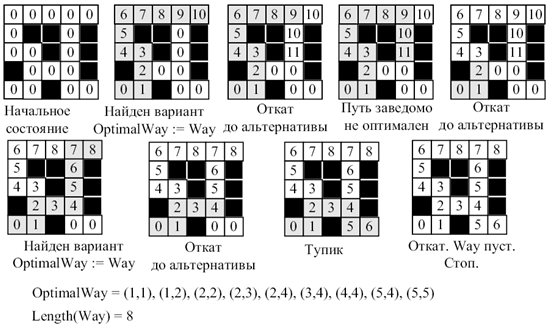
\includegraphics[width=13cm]{pic/45_03.png}
\end{figure}
\begin{lstlisting}
[label=code:pe,caption=Опис функції переборного алгоритму методом пошуку в глибину]
 / * Опис функції переборного алгоритму методом пошуку в глибину * /
void Backtracking (int n, int m, int ** Maze) {
  int Begin, End, Current;
  Begin = (n - 1) * m;
  End = m - 1;
  int * Way, * OptimalWay;
  int LengthWay, LengthOptimalWay;
  Way = new int [n * m];
  OptimalWay = new int [n * m];
  LengthWay = 0;
  LengthOptimalWay = m * n;
  for (int i = 0; i <n * m; i ++)
    Way [i] = OptimalWay [i] = -1;
  int * Dist;
  Dist = new int [n * m];
  for (int i = 0; i <n; i ++)
    for (int j = 0; j <m; j ++)
      Dist [i * m + j] = (Maze [i] [j] == 0? 0: -1);
  Way [LengthWay ++] = Current = Begin;
  while (LengthWay> 0) {
    if (Current == End) {
      if (LengthWay <LengthOptimalWay) {
        for (int i = 0; i <LengthWay; i ++)
          OptimalWay [i] = Way [i];
        LengthOptimalWay = LengthWay;
       }
      if (LengthWay> 0) Way [- LengthWay] = -1;
      Current = Way [LengthWay-1];
     }
    else {
      int Neighbor = -1;
      if ((Current / m - 1)> = 0 &&! Insert (Way, Current - m) &&
        (Dist [Current - m] == 0 || Dist [Current - m]> LengthWay)
        && Dist [Current] <LengthOptimalWay)
          Neighbor = Current - m;
       else 
        if ((Current% m - 1)> = 0 &&! Insert (Way, Current - 1) &&
          (Dist [Current - 1] == 0 || Dist [Current - 1]> LengthWay)
          && Dist [Current] <LengthOptimalWay)
            Neighbor = Current - 1;
         else 
          if ((Current% m + 1) <m &&! Insert (Way, Current + 1) &&
           (Dist [Current + 1] == 0 || Dist [Current + 1]> LengthWay)
          && Dist [Current] <LengthOptimalWay)
            Neighbor = Current + 1;
          else 
           if ((Current / m + 1) <n &&! Insert (Way, Current + m) &&
            (Dist [Current + m] == 0 || Dist [Current + m]> LengthWay)
           && Dist [Current] <LengthOptimalWay)
             Neighbor = Current + m;
      if (Neighbor! = -1) {
        Way [LengthWay ++] = Neighbor;
        Dist [Neighbor] = Dist [Current] + 1;
        Current = Neighbor;
       }
       else {
        if (LengthWay> 0) Way [- LengthWay] = -1;
        Current = Way [LengthWay-1];
       }
     }
   }
  if (LengthOptimalWay <n * m) 
    cout << endl << "Yes. Length way =" << LengthOptimalWay << endl;
  else cout << endl << "No" << endl;
 } 
\end{lstlisting}


\subsection{Хвильовий алгоритм}

Цей переборний алгоритм, який заснований на пошуку в ширину, складається з двох етапів:
\begin{itemize}
\item поширення хвилі;
\item зворотний хід.
\end{itemize}
 
Поширення хвилі і є власне пошук в ширину, при якому клітини позначаються номером кроку методу, на якому клітина відвідується. При зворотному ході, починаючи з кінцевої вершини, йде відновлення шляху, по якому в неї потрапили шляхом включення до нього клітин з мінімальною позначкою (рис.~\ref{pic:45.4}). Важливою особливістю є те, що відновлення починається з кінця (з початку воно найчастіше неможливо).
Демонстрація хвильового алгоритму

\begin{figure}
\caption{Демонстрація хвильового алгоритму}\label{pic:45.4}
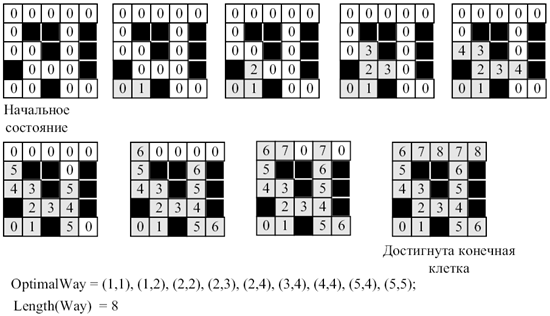
\includegraphics[width=13cm]{pic/45_04.png}
\end{figure}


Зауважимо, що перебір методом пошуку в ширину в порівнянні з перебором з поверненням, як правило, вимагає більше допоміжної пам'яті, яка необхідна для зберігання інформації, щоб побудувати шлях при зворотному ході і помітити відвідані вершини. Однак він працює швидше, оскільки абсолютно виключається відвідування однієї і тієї ж клітини більш ніж один раз.

\section{Приклади обчислень}
\nopagebreak[4]




\subsection*{Контрольні запитання}
\nopagebreak[4]
\begin{enumerate}
\item ?
\end{enumerate}




%\chapter{Використання багаторозгалужених дерев}
\nopagebreak[4]
\section*{Мета роботи}

\nopagebreak[4]
\section{Вступ}
\nopagebreak[4]


\section{Ключові терміни}
\nopagebreak[4]




\section{Розширені теоретичні відомості}
\nopagebreak[4]




\section{Приклади обчислень}
\nopagebreak[4]




\subsection*{Контрольні запитання}
\nopagebreak[4]
\begin{enumerate}
\item ?
\end{enumerate}




%\chapter{Алгоритми сортування}


\nopagebreak[4]
\section{Вступ}
\nopagebreak[4]
\textbf{Алгоритмом сортування} називається алгоритм для впорядкування деякого безлічі елементів. Зазвичай під алгоритмом сортування подразумевают алгоритм упорядкування безлічі елементів за зростанням або спаданням.

У разі наявності елементів з однаковими значеннями, у впорядкованій послідовності вони розташовуються поруч один за одним у будь-якому порядку. Однак іноді буває корисно зберігати первісний порядок елементів з однаковими значеннями.

Алгоритми сортування мають велике практичне застосування. Їх можна зустріти там, де мова йде про обробку та зберіганні великих обсягів інформації. Деякі завдання обробки даних вирішуються простіше, якщо дані заздалегідь впорядкувати.

\section{Ключові терміни}
\nopagebreak[4]




\section{Розширені теоретичні відомості}
\nopagebreak[4]
В алгоритмах сортування лише частина даних використовується як ключ сортування. Ключем сортування називається атрибут (або декілька атрибутів), за значенням якого визначається порядок елементів. Таким чином, при написанні алгоритмів сортувань масивів слід врахувати, що ключ повністю або частково збігається з даними.

Практично кожен алгоритм сортування можна розбити на 3 частини:
\begin{enumerate}
\item порівняння, визначальне впорядкованість пари елементів;
\item перестановку, змінюють місце пару елементів;
\item власне сортують алгоритм, який здійснює порівняння і перестановку елементів до тих пір, поки всі елементи множини не будуть впорядковані.
\end{enumerate}

\subsection{Оцінка алгоритмів сортування}

Жодна інша проблема не породила такої кількості найрізноманітніших рішень, як завдання сортування. Універсального, найкращого алгоритму сортування на даний момент не існує. Проте, маючи приблизні характеристики вхідних даних, можна підібрати метод, який працює оптимальним чином. Для цього необхідно знати параметри, за якими буде проводитися оцінка алгоритмів.

\textbf{Час сортування} - основний параметр, що характеризує швидкодію алгоритму.

\textbf{Пам'ять} - один з параметрів, який характеризується тим, що ряд алгоритмів сортування вимагають виділення додаткової пам'яті під тимчасове зберігання даних. При оцінці використовуваної пам'яті не враховуватиметься місце, яке займає вихідний масив даних і незалежні від вхідної послідовності витрати, наприклад, на зберігання коду програми.

\textbf{Стійкість} - це параметр, який відповідає за те, що сортування не змінює взаємного розташування рівних елементів.

\textbf{Природність поведінки} - параметр, якій вказує на ефективність методу при обробці вже відсортованих, або частково відсортованих даних. Алгоритм поводиться природно, якщо враховує цю характеристику вхідної послідовності і працює краще.

\subsection{Класифікація алгоритмів сортувань}

Все розмаїття і різноманіття алгоритмів сортувань можна класифікувати за різними ознаками, наприклад, по стійкості, по поведінці, по використанню операцій порівняння, за потреби в додатковій пам'яті, по потреби в знаннях про структуру даних, що виходять за рамки операції порівняння, та інші.

Найбільш докладно розглянемо класифікацію алгоритмів сортування за сферою застосування. У даному випадку основні типи впорядкування діляться наступним чином.

\textbf{Внутрішнє сортування} - це алгоритм сортування, який в процесі упорядкування даних використовує тільки оперативну пам'ять (ОЗП) на комп'ютері. Тобто оперативної пам'яті достатньо для завантаження в неї сортованого масиву даних з довільним доступом до будь-якій комірці і власне для виконання алгоритму. Внутрішня сортування застосовується у всіх випадках, за винятком однопрохідного зчитування даних і однопрохідної записи відсортованих даних. Залежно від конкретного алгоритму та його реалізації дані можуть сортуватися в тій же області пам'яті, або використовувати додаткову оперативну пам'ять.

\textbf{Зовнішнє сортування} - це алгоритм сортування, який при проведенні упорядкування даних використовує зовнішню пам'ять, як правило, жорсткі диски. Зовнішня сортування розроблена для обробки великих списків даних, які не поміщаються в оперативну пам'ять. Звернення до різних носіям накладає деякі додаткові обмеження на даний алгоритм: доступ до носія здійснюється послідовним чином, тобто в кожен момент часу можна вважати або записати тільки елемент, наступний за поточним; обсяг даних не дозволяє їм розміститися в ОЗУ.

Внутрішнє сортування є базовою для будь-якого алгоритму зовнішньої сортування - окремі частини масиву даних сортуються в оперативної пам'яті і за допомогою спеціального алгоритму зчіплюються в один масив, упорядкований по ключу.







%\chapter{Алгоритми внутрішнього сортування}
\nopagebreak[4]
\section*{Мета роботи}

\nopagebreak[4]
\section{Вступ}
\nopagebreak[4]


\section{Ключові терміни}
\nopagebreak[4]




\section{Розширені теоретичні відомості}
\nopagebreak[4]




\section{Приклади обчислень}
\nopagebreak[4]




\subsection*{Контрольні запитання}
\nopagebreak[4]
\begin{enumerate}
\item ?
\end{enumerate}




%\chapter{Алгоритми зовнішнього сортування}


\nopagebreak[4]
\section{Вступ}
\nopagebreak[4]
\textbf{Зовнішнє сортування} - сортування даних, розташованих на периферійних пристроях і не вміщаються в оперативну пам'ять, тобто коли застосувати одну з внутрішніх сортувань неможливо. Варто відзначити, що внутрішня сортування значно ефективніше зовнішньої, так як на звернення до оперативної пам'яті витрачається набагато менше часу, ніж до магнітних дисків, стрічок і т.п.

Найбільш часто зовнішнє сортування використовується в СУБД.

Дані, що зберігаються на зовнішніх пристроях, мають великий обсяг, що не дозволяє їх цілком перемістити в оперативну пам'ять, відсортувати з використанням одного з алгоритмів внутрішнього сортування, а потім повернути їх на зовнішній пристрій. У цьому випадку здійснювалося б мінімальну кількість проходів через файл, тобто було б однократне читання і однократна запис даних. Однак на практиці доводиться здійснювати читання, обробку і запис даних у файл по блоках, розмір яких залежить від операційної системи та наявного обсягу оперативної пам'яті, що призводить до збільшення числа проходів через файл і помітного зниження швидкості сортування.

\section{Ключові терміни}
\nopagebreak[4]
\textbf{Зовнішнє сортування} - це сортування даних, які розташовані на зовнішніх пристроях і не вміщаються в оперативну пам'ять.

\textbf{Фаза} - це дії по одноразовій обробці всієї послідовності елементів.

\textbf{Серія (упорядкований відрізок)} - це послідовність елементів, що упорядкована по ключу. Кількість елементів в серії називається довжиною серії.

\textbf{Двофазне сортування} - це сортування, в якому окремо реалізується дві фази: розподіл і злиття. 

\textbf{Однофазне сортування} - це сортування, в якому об'єднані фази розподілу і злиття в одну.

\textbf{Двоколійним злиттям} називається сортування, в якому дані розподіляються на два допоміжних файли. 

\textbf{Багатоколійним злиттям} називається сортування, в якому дані розподіляються на N (N> 2) допоміжних файлів.



\section{Розширені теоретичні відомості}
\nopagebreak[4]

\subsection{Сортування простим злиттям}

Одне з сортувань на основі злиття називається простим злиттям.

Алгоритм сортування простим злиття є найпростішим алгоритмом зовнішньої сортування, заснований на процедурі злиття серією.

У даному алгоритмі довжина серій фіксується на кожному кроці. У вихідному файлі всі серії мають довжину 1, після першого кроку вона дорівнює 2, після другого - 4, після третього - 8, після k-го кроку - 2k.

Алгоритм сортування простим злиттям

\begin{enumerate}
\item Вихідний файл f розбивається на два допоміжних файлу f1 і f2.

\item Допоміжні файли f1 і f2 зливаються в файл f, при цьому поодинокі елементи утворюють впорядковані пари.

\item Отриманий файл f знову обробляється, як зазначено в кроках 1 і 2. При цьому впорядковані пари переходять у впорядковані четвірки.

\item Повторюючи кроки, зливаємо четвірки в вісімки і т.д., кожен раз подвоюючи довжину злитих послідовностей до тих пір, поки не буде впорядкований цілком весь файл (рис.~\ref{f:sort1}).
\end{enumerate}

\begin{figure}
\caption{Демонстрація сортування двоколійному двофазним простим злиттям}\label{f:sort1}
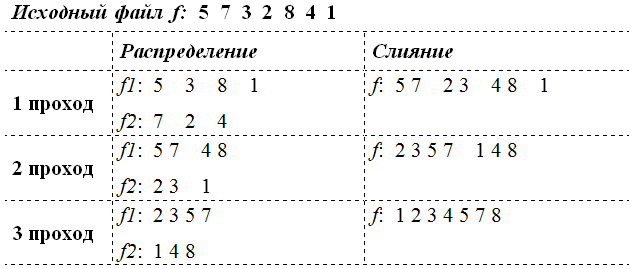
\includegraphics[width=13cm]{pic/43_01.png}

\end{figure}

Після виконання i проходів отримуємо два файли, що складаються з серій довжини 2i. Закінчення процесу відбувається при виконанні умови $2^i \geq n$. Отже, процес сортування простим злиттям вимагає порядку $O (\log n)$ проходів за даними.

Ознаками кінця сортування простим злиттям є наступні умови:

\begin{enumerate}
\item довжина серії не менша кількість елементів у файлі (визначається після фази злиття);
\item кількість серій рівно 1 (визначається на фазі злиття).
\item при однофазному сортуванні другий за рахунком допоміжний файл після розподілу серій залишився порожнім.
\end{enumerate}

Приклад програмної реалізації надано у додатку \ref{code:sort111};

\section{Приклади обчислень}
\nopagebreak[4]







%\chapter{Характеристика алгоритмів порівняння методів сортування}
\nopagebreak[4]
\section*{Мета роботи}

\nopagebreak[4]
\section{Вступ}
\nopagebreak[4]


\section{Ключові терміни}
\nopagebreak[4]




\section{Розширені теоретичні відомості}
\nopagebreak[4]




\section{Приклади обчислень}
\nopagebreak[4]




\subsection*{Контрольні запитання}
\nopagebreak[4]
\begin{enumerate}
\item ?
\end{enumerate}




\appendix
\makeatletter
\gdef\thechapter{\@Asbuk\c@chapter}
\makeatother
\def\chaptername{Додаток}


\chapter{Правила оформлення звіту}
\section{Титульна сторінка лабораторної роботи}
%\begin{titlepage}
%\newpage

\hrulefill

\begin{center}
МІНІСТЕРСТВО ОСВІТИ І НАУКИ, МОЛОДІ ТА СПОРТУ УКРАЇНИ \\

ХЕРСОНСЬКИЙ НАЦІОНАЛЬНИЙ ТЕХНІЧНИЙ УНІВЕРСИТЕТ \\*

КАФЕДРА ІНФОРМАЦІЙНИХ ТЕХНОЛОГІЙ

\end{center}

\vspace{5em}

\begin{center}
\Large Звіт до лабораторної роботи \No 123 \\ з дисципліни <<Web-програмування>>
\end{center}

\vspace{2.5em}

\begin{center}
{\Large Тема: \textbf{<<Основи мережі Internet>>}}
\end{center}

\vspace{5em}





\begin{flushleft}
Виконав \\ст.групи хПР1 \hspace{\fill} Пупкін А.А. \\
\vspace{1em}
Перевірив \\ст.викладач \hspace{\fill} Іванов Б.Б.\\
\end{flushleft}

\vspace{\fill}

\begin{center}
Херсон 2012
\end{center}
\newpage
%\end{titlepage}
\section{Приклади блок-схем}
Правила виконання блок-схем задані наступними документами:
\begin{itemize}
\item ГОСТ 19.701-90. Схемы алгоритмов, программ, данных и систем. Условные обозначения и правила выполнения
\item ГОСТ 19.002-80. Схемы алгоритмов и программ. Правила выполнения
\item ГОСТ 19.003-80. Схемы алгоритмов и программ. Обозначения условные графические

\end{itemize}



%\include{ap02}
%\include{ap03}
%\include{ap04}
%\include{ap05}
%\include{ap06}
%\include{ap07}
%\include{ap08}
%\include{ap09}
%\include{ap10}
 
 



%% указываем класс документа
%\documentclass[twoside,8pt,a5paper,openany]{report}
\documentclass[twoside,12pt,a4paper,openany]{report}

% подключаем собственный стилевой файл
\usepackage{labstyle}
\usepackage{labstyle2}







\makeindex





\begin{document}


% указываем язык (для автоматической вставки слов, типа "Глава", "Содержание", "Литература", "рис." и пр.
\selectlanguage{ukrainian}



% подключаем файлы содержимого
\begin{titlepage}
\newpage

\begin{center}
МІНІСТЕРСТВО ОСВІТИ І НАУКИ УКРАЇНИ \\

ХЕРСОНСЬКИЙ ПОЛІТЕХНІЧНИЙ КОЛЕДЖ \\

ОДЕСЬКОГО НАЦІОНАЛЬНОГО ПОЛІТЕХНІЧНОГО УНІВЕРСИТЕТУ\\

ВІДДІЛЕННЯ КОМП'ЮТЕРНОЇ ТА ПРОГРАМНОЇ ІНЖЕНЕРІЇ

\end{center}


\vspace{10em}

\begin{center}
\Large Курс лекції \\ з дисципліни
\end{center}

\vspace{2em}

\begin{center}
\huge{\textbf{<<Алгоритми та структури даних>>}}
\end{center}




\vspace{\fill}

\begin{center}
Херсон --- 2015
\end{center}

\end{titlepage}



% ненужное можно просто закомментировать знаком процента "%" 

% первую страницу не нумеруем
%\thispagestyle{empty}			

% название
%\title{Методичні вказівки до лабораторних робіт з дисципліни <<web-програмування>>}
%\author{Жарікова М.В., Левицький В.М.}
%\maketitle

% печатаем содержание
%\chapter*[Зміст]{Зміст}
\tableofcontents

% ничанаем с новой страницы
%\newpage

% печатаем перечень рисунков
%\chapter*{Перелік ілюстрацій}
\listoffigures

% печатаем перечень таблиц
%\chapter*{Перелік таблиць}
\listoftables

\lstlistoflistings

%\lstlistoflistings


\chapter{Рекурсія і рекурсивні алгоритми}
\nopagebreak[4]
\section*{Мета роботи}
Вивчити поняття, види рекурсії і рекурсивну тріаду, навчитися розробляти рекурсивну тріаду при вирішенні завдань мовою C++.

При виконанні лабораторної роботи для кожного завдання потрібно написати програму на мові С++, яка отримує на вході числові дані, виконує їх обробку відповідно до вимог завдання і виводить результат на екран. Для обробки даних необхідно реалізувати рекурсивну функцію. Введення даних здійснюється з клавіатури з урахуванням вимог до вхідних даних, що містяться в постановці завдання (введення даних супроводжуйте діалогом). Обмеженнями на вхідні дані є допустимий діапазон значень використовуваних числових типів в мові С++.

\nopagebreak[4]
\section{Теоретичнi вiдомостi}

\begin{lstlisting}[label=code:rec1,caption=Програма обчислення факторіалу ітераційним способом]
public class App {
    public static void main(String[] args) {
        System.out.println(factorial(5));
    }
     
    public static int factorial(int arg) {
        int result = 1;
        for (int k = 1; k <= arg; k++) {
            result *= k;
        }
        return result;
    }
}
 
>> 120
\end{lstlisting}

\begin{lstlisting}[label=code:rec1,caption=Програма обчислення факторіалу рекурсивним способом]
public class App {
    public static void main(String[] args) {
        System.out.println(factorial(5));
    }
     
    public static int factorial(int arg) {
        if (arg == 1) {
            return 1;
        } else {
            return arg * factorial(arg - 1);
        }
    }
}
 
>> 120
\end{lstlisting}
\nopagebreak[4]
\section{Вказівки до виконання роботи.}
\nopagebreak[4]

Кожне завдання необхідно вирішити вивченими рекурсивними методами вирішення завдань і методами обробки числових даних у мові С++. Перед реалізацією коду кожного завдання необхідно розробити рекурсивну тріаду відповідно до постановкою завдання: виконати параметризацію, виділити базу і оформити декомпозицію рекурсії. Програму для вирішення кожного завдання необхідно розробити методом процедурної абстракції, використовуючи рекурсивні функції. Етапи супроводити коментарями в коді.

Слід реалізувати кожне завдання у відповідності з наведеними етапами:

\begin{itemize}
\item вивчити словесну постановку задачі, виділивши при цьому всі види даних;
\item сформулювати математичну постановку задачі;
\item вибрати метод розв'язання задачі, якщо це необхідно;
\item розробити графічну схему алгоритму;
\item записати розроблений алгоритм на мові С ++;
\item розробити контрольний тест до програми;
\item налагодити програму;
\item подати звіт по роботі. 
\end{itemize}



\section{Індивідуальне завдання}
\nopagebreak[4]
\subsection*{Завдання до лабораторної роботи}
\nopagebreak[4]
\begin{enumerate}
\item Створіть програму для обчислення $n$-го числі Фібоначчі.

\end{enumerate}

\subsection*{Контрольні запитання}
\nopagebreak[4]
\begin{enumerate}
\item Чи можна випадок непрямої рекурсії звести до прямої рекурсії? Відповідь обґрунтуйте.
\item Чи може рекурсивна база містити кілька тривіальних випадків? Відповідь обґрунтуйте.
\item Чи є параметри, база і декомпозиція єдиними для конкретного завдання? Відповідь обґрунтуйте.
\item З якою метою в задачах відбувається перегляд або коригування обраних параметрів, виділеної бази або випадку декомпозиції?
\item Чи є рекурсія універсальним способом вирішення завдань? Відповідь обґрунтуйте.
\item Чому для оцінки трудомісткості рекурсивного алгоритму недостатньо одного методу підрахунку вершин рекурсивного дерева?


\end{enumerate}




\chapter{Рекурсія}
\nopagebreak[4]
\section*{Мета роботи}

\nopagebreak[4]
\section{Вступ}
\nopagebreak[4]
У математиці для вирішення переважної більшості завдань використовуються методи, які в кінцевому рахунку можуть бути зведені до одного з двох базових способів: ітерації або рекурсії.


\textbf{Ітерація} означає кількаразове повторення одних і тих же дій, яке після деякої кількості кроків приводить до бажаного результату. Характерним прикладом ітераційного способу вирішення завдання є методи послідовних наближень рішення нелінійних рівнянь, у тому числі метод дотичних, метод хорд і т.д.

\begin{equation}
f(x)=0; x=\varphi(x); x_0=a; x_n=\varphi(x_{n-1}), n=1,2,..., |x_k-x_{k-1}|>\epsilon
\end{equation}

\textbf{Рекурсія} являє собою посилання при описі об'єкта, дії на описуваний об'єкт, дія. Рекурсія означає рішення задачі за допомогою відомості рішення до самого себе. При цьому обчислення залежать від інших, в не-якому сенсі більш простих (зазвичай менших) значень аргументу або аргументів завдання. Повністю аналогічні механізми використовуються в базовій теорії рекурсивних функцій, у методі математичної індукції, а також в рекурентних послідовностях. 

Наприклад:

\begin{equation}
a_k = 2a_{k-1} + k , \forall k > 0, a_0 = 1
\end{equation}

\textbf{Рекурсивний алгоритм} - це алгоритм, в описі якого прямо або побічно міститься звернення до самого себе. У техніці процедурного програмування дане поняття поширюється на функцію, яка реалізує рішення окремого блоку завдання за допомогою виклику зі свого тіла інших функцій, в тому числі і себе самої. Якщо при цьому на черговому етапі роботи функція організовує звернення до самої себе, то така функція є рекурсивної.



\section{Ключові терміни}
\nopagebreak[4]


\textbf{База рекурсії} - це тривіальний випадок, при якому рішення задачі очевидно, тобто не потрібно звернення функції до себе.

\textbf{Глибина рекурсивних викликів} - це найбільше одночасне кількість рекурсивних звернень функції, визначальне максимальну кількість шарів рекурсивного стека.

\textbf{Декомпозиція} - це вираження загального випадку через більш прості підзадачі зі зміненими параметрами.

\textbf{Корінь повного дерева рекурсивних викликів} - це вершина повного дерева рекурсії, відповідна початкового зверненням до функції.

\textbf{Непряма (взаємна) рекурсія} - це послідовність взаємних викликів декількох функцій, організована у вигляді циклічного замикання на тіло первісної функції, але з іншим набором параметрів.

\textbf{Обсяг рекурсії} - це характеристика складності рекурсивних обчислень для конкретного набору параметрів, що представляє собою кількість вершин повного рекурсивного дерева без одиниці.

\textbf{Параметризація} - це виділення з постановки задачі параметрів, які використовуються для опису умови задачі і рішення.

\textbf{Повне дерево рекурсії} - це граф, вершинами якого є набори фактичних параметрів при всіх викликах функції, починаючи з першого звернення до неї, а ребрами - пари таких наборів, відповідних взаємним викликам.

\textbf{Пряма рекурсія} - це безпосереднє звернення рекурсивної функції до себе, але з іншим набором вхідних даних.

\textbf{Рекурсивна тріада} - це етапи вирішення завдань рекурсивним методом.

\textbf{Рекурсивна функція} - це функція, яка у своєму тілі містить звернення до самої себе зі зміненим набором параметрів.

\textbf{Рекурсивний алгоритм} - це алгоритм, у визначенні якого міститься прямий або непрямий виклик цього ж алгоритму.

\textbf{Рекурсія} - це визначення об'єкта за допомогою посилання на себе.


\section{Розширені теоретичні відомості}
\nopagebreak[4]


Рекурсивні алгоритми зазвичай виходять на основі математичної постановки завдання. Найважливіше при побудові рекурсивного алгоритму: побачити однакові дії на поточному та попередньому кроці обчислень (дій).

Виконавець рекурсивного алгоритму зводить невідоме до іншого невідомого, накопичуючи інформацію (прямий хід) і відкладаючи фактичні обчислення до моменту, коли виконається умова, що дозволяють безпосередньо обчислити шукане значення. Потім виконується зворотний хід рекурсії.

\textbf{Основні переваги рекурсії:}
\begin{itemize}
\item простота математичного формулювання;
\item простота алгоритму і його реалізації
\end{itemize}
\textbf{Основні недоліки рекурсії:}
\begin{itemize}
\item додаткові витрати оперативної пам'яті;
\item додаткові тимчасові витрати;
\item можливий перехід складності в клас EXP.
\end{itemize}

За аналогією з математичної індукцією, на яку рекурсія трохи схожа, будь рекурсивна процедура повинна включати в себе базис і крок рекурсії.

Базис рекурсії - це пропозиція, що визначає якусь початкову ситуацію або ситуацію в момент припинення. Як правило, в цій пропозиції записується якийсь найпростіший випадок, при якому відповідь виходить відразу навіть без використання рекурсії. Так, у наведеній вище процедурі, яка описує предикат предок, базисом рекурсії є перше правило, в якому визначено, що найближчими предками людини є його батьки. Ця пропозиція часто містить умову, при виконанні якї відбувається вихід з рекурсії або відсікання.

Крок рекурсії - це правило, в тілі якого обов'язково міститься, в якості підцілі, виклик обумовленого предиката. Якщо ми хочемо уникнути зациклення, який визначається предикат повинен викликатися не вiд тих же параметрів, які вказані в заголовку правила. Параметри повинні змінюватися на кожному кроці так, щоб в результаті або спрацював базис рекурсії, або умова виходу з рекурсії, розміщене в самому правилі.

\section{Приклади обчислень}
\nopagebreak[4]


\subsection*{Приклад 1. Обчислення факторіала $P=n!$, n - ціле число}

Зазвичай для обчислення факторіала цілого числа використовується ітераційний спосіб, заснований на багаторазовому домноженні величини, в якій накопичується результат, на черговий співмножник: 

\begin{equation}
Pi := P_{i-1} \times i, i=2,3,...,k.  
\end{equation}

\begin{lstlisting}[label=iter1,caption=Ітераційна функція] 
function factorial (k:integer):integer;
	var P,i:integer;  { i – номер сомножителя, P – накапливаемый результат}
begin
	P:=1;
	for i:=1 to k do
		P:=P*i;
	factorial:=P;
end;
\end{lstlisting}

Це завдання можна вирішити і за допомогою рекурсії, базуючись на наступних міркуваннях:

\begin{equation}
k! = 1 \times 2 \times 3 \times \dots \times k =  1 \times 2 \times 3 \times \dots \times (k-1) \times k = (k-1)! \times k
\end{equation}

Отже, $P(k) = k!$ можна визначити таким чином:

\begin{equation}
P(k) = 
 \begin{cases}
   1,k=1\\
   P(k-1)\times k,k>1
 \end{cases}
\end{equation}

\begin{lstlisting}[label=iter1,caption=Рекурентна функція] 
function factorial1 (k:integer):integer ;
begin
	if k=1 then factorial1:=1 
		else  factorial1:= factorial1(k-1)*k
end;
\end{lstlisting}




\section{Індивідуальне завдання}
\nopagebreak[4]
\subsection*{Завдання до лабораторної роботи}
\nopagebreak[4]
\begin{enumerate}
\item Вивчити теоретичний матеріал
\item Відповісти на контрольні запитання
\item Скласти звіт
\item Захистити роботу
\end{enumerate}

\subsection*{Контрольні запитання}
\nopagebreak[4]
\begin{enumerate}
\item Що таке Internet? З яких структурних частин складається Internet?
\item Що таке IP-адреса?
\item Що таке доменне ім'я, з чого воно складається?
\item Який сервіс Internet перетворює IP-адреси в доменні імена і навпаки?
\item Яка служба займається розподіленням блоків IP-адрес?
\item Протокол HTTP. Рівень у моделі OSI, призначення.
\item Значення URI, URL, URN.
\item Мови web-програмування, які ви знаєте.
\item Веб-сервери, які ви знаєте.
\item Мережеві СКБД, які ви знаєте. 
\end{enumerate}




\chapter{Представлення виразів за допомогою дерев}
\nopagebreak[4]
\section*{Мета роботи}

\nopagebreak[4]
\section{Вступ}
\nopagebreak[4]


\section{Ключові терміни}
\nopagebreak[4]




\section{Розширені теоретичні відомості}
\nopagebreak[4]




\section{Приклади обчислень}
\nopagebreak[4]




\subsection*{Контрольні запитання}
\nopagebreak[4]
\begin{enumerate}
\item ?
\end{enumerate}
%\chapter{Представлення багаторозгалужених дерев}
\nopagebreak[4]
\section*{Мета роботи}

\nopagebreak[4]
\section{Вступ}
\nopagebreak[4]


\section{Ключові терміни}
\nopagebreak[4]




\section{Розширені теоретичні відомості}
\nopagebreak[4]




\section{Приклади обчислень}
\nopagebreak[4]




\subsection*{Контрольні запитання}
\nopagebreak[4]
\begin{enumerate}
\item ?
\end{enumerate}




%\chapter{Представлення графів}
\nopagebreak[4]
\section*{Мета роботи}

\nopagebreak[4]
\section{Вступ}
\nopagebreak[4]


\section{Ключові терміни}
\nopagebreak[4]




\section{Розширені теоретичні відомості}
\nopagebreak[4]




\section{Приклади обчислень}
\nopagebreak[4]




\subsection*{Контрольні запитання}
\nopagebreak[4]
\begin{enumerate}
\item ?
\end{enumerate}



 
%\chapter{Алгоритми на графах}
\nopagebreak[4]

\section{Вступ}
\nopagebreak[4]
Знаходження найкоротшого шляху на сьогоднішній день є життєво необхідним завданням і використовується практично скрізь, починаючи від знаходження оптимального маршруту між двома об'єктами на місцевості (наприклад, найкоротший шлях від будинку до університету), в системах автопілота, для знаходження оптимального маршруту при перевезеннях, комутації інформаційного пакету в мережах і т.п.

Найкоротший шлях розглядається за допомогою деякого математичного об'єкта, званого графом. Пошук найкоротшого шляху ведеться між двома заданими вершинами в графі. Результатом є шлях, тобто послідовність вершин і ребер, інцидентних двом сусіднім вершинам, і його довжина.

Розглянемо три найбільш ефективних алгоритму знаходження найкоротшого шляху:

\begin{itemize}
\item алгоритм Дейкстри;
\item алгоритм Флойда;
\item Переборні алгоритми. 
\end{itemize}

Зазначені алгоритми легко виконуються при малій кількості вершин у графі. При збільшенні їх кількості завдання пошуку найкоротшого шляху ускладнюється. 




\section{Ключові терміни}
\nopagebreak[4]
\textbf{Алгоритм Дейкстри} - це алгоритм знаходження найкоротшого шляху від однієї з вершин графа до всіх інших, який працює тільки для графів без ребер негативного ваги.

\textbf{Алгоритм Флойда} - це алгоритм пошуку найкоротшого шляху між будь-якими двома вершинами графа.

\textbf{Хвильовий алгоритм} - це переборний алгоритм, який заснований на пошуку в ширину і складається з двох етапів: поширення хвилі і зворотний хід.

\textbf{Найкоротший шлях} - це шлях в графі, тобто послідовність вершин і ребер, інцидентних двом сусіднім вершинам, і його довжина.

Переборний алгоритм - це алгоритм обходу графа, заснований на послідовному переборі можливих шляхів.



\section{Розширені теоретичні відомості}
\subsection{Алгоритм Дейкстри}
\nopagebreak[4]

Даний алгоритм є алгоритмом на графах, який винайдений нідерландським вченим Е. Дейкстрой в 1959 році. Алгоритм знаходить найкоротший відстань від однієї з вершин графа до всіх інших і працює тільки для графів без ребер негативного ваги.

Кожній вершині приписується вага - це вага шляху від початкової вершини до даної. Також кожна вершина може бути виділена. Якщо вершина виділена, то шлях від неї до початкової вершини найкоротший, якщо ні - то тимчасовий. Обходячи граф, алгоритм вважає для кожної вершини маршрут, і, якщо він виявляється найкоротшим, виділяє вершину. Вагою даної вершини стає вага шляху. Для всіх сусідів даної вершини алгоритм також розраховує вагу, при цьому ні за яких умов не виділяючи їх. Алгоритм закінчує свою роботу, дійшовши до кінцевої вершини, і вагою найкоротшого шляху стає вага кінцевої вершини.

Алгоритм Дейкстри
\begin{enumerate}
\item Всім вершинам, за винятком першої, присвоюється вага рівний нескінченності, а першій вершині - 0.

\item Всі вершини не виділені.

\item Перша вершина оголошується поточної.

\item Вага всіх невиділених вершин перераховується за формулою: вага невиділеної вершини є мінімальне число зі старого ваги даної вершини, суми ваги поточної вершини і ваги ребра, що з'єднує поточну вершину з невиділеної.

\item Серед невиділених вершин шукається вершина з мінімальною вагою. Якщо така не знайдена, тобто вага всіх вершин дорівнює нескінченності, то маршрут не існує. Отже, вихід. Інакше, поточної стає знайдена вершина. Вона ж виділяється.

\item Якщо поточною вершиною виявляється кінцева, то шлях знайдений, і його вага є вага кінцевої вершини.

\item Перехід на крок 4.
\end{enumerate}

У програмній реалізації алгоритму Дейкстри побудуємо безліч S вершин, для яких найкоротші шляхи від початкової вершини вже відомі. На кожному кроці до множини S додається та з решти вершин, відстань до якої від початкової вершини менше, ніж для інших, що залишилися вершин. При цьому будемо використовувати масив D, в який записуються довжини найкоротших шляхів для кожної вершини. Коли безліч S буде містити всі вершини графа, тоді масив D міститиме довжини найкоротших шляхів від початкової вершини до кожної вершини.

Крім зазначених масивів будемо використовувати матрицю довжин C, де елемент C [i, j] - довжина ребра (i, j), якщо ребра немає, то її довжина покладається рівною нескінченності, тобто більше будь фактичної довжини ребер. Фактично матриця C являє собою матрицю суміжності, в якій всі нульові елементи замінені на нескінченність.

Для визначення самого найкоротшого шляху введемо масив P вершин, де P [v] буде містити вершину, безпосередньо попередню вершині v в найкоротшому шляху (рис.~\ref{pic:45.1}).
Демонстрація алгоритмом Дейкстри
\begin{figure}
\caption{Демонстрація алгоритму Дейкстри}\label{pic:45.1}
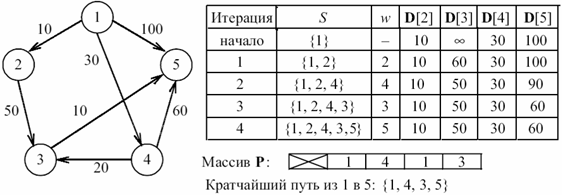
\includegraphics[width=13cm]{pic/45_01.png}

\end{figure}

\begin{lstlisting}[label=code:de,caption=Опис функції алгоритму Дейкстри]
  // Опис функції алгоритму Дейкстри
void Dijkstra (int n, int ** Graph, int Node) {
   bool * S = new bool [n];
   int * D = new int [n];
   int * P = new int [n];
   int i, j;
   int Max_Sum = 0;
   for (i = 0; i <n; i ++)
     for (j = 0; j <n; j ++)
       Max_Sum + = Graph [i] [j];
   for (i = 0; i <n; i ++)
     for (j = 0; j <n; j ++)
       if (Graph [i] [j] == 0) 
         Graph [i] [j] = Max_Sum;
   for (i = 0; i <n; i ++) {
     S [i] = false;
     P [i] = Node;
     D [i] = Graph [Node] [i];
   }
   S [Node] = true;
   P [Node] = -1;
   for (i = 0; i <n - 1; i ++) {
     int w = 0;
     for (j = 1; j <n; j ++) {
       if (! S [w]) {
         if (! S [j] && D [j] <= D [w])
           w = j;
       }
       else w ++;
     }
     S [w] = true;
     for (j = 1; j <n; j ++)
       if (! S [j])
         if (D [w] + Graph [w] [j] <D [j]) {
           D [j] = D [w] + Graph [w] [j];
           P [j] = w;
         }
   }
   for (i = 0; i <n; i ++)
     printf ("% 5d", D [i]);
   cout << endl;
   for (i = 0; i <n; i ++)
     printf ("% 5d", P [i] +1);
   cout << endl;
   delete [] P;
   delete [] D;
   delete [] S;
 } 
\end{lstlisting}

Складність алгоритму Дейкстри залежить від способу знаходження вершини, а також способу зберігання безлічі невідвіданих вершин і способи оновлення довжин.

Якщо для представлення графа використовувати матрицю суміжності, то час виконання цього алгоритму має порядок O (n 2), де n - кількість вершин графа. 

\subsection{Алгоритм Флойда}
Розглянутий алгоритм іноді називають алгоритмом Флойда -Уоршелла. Алгоритм Флойда -Уоршелла є алгоритмом на графах, який розроблений в 1962 році Робертом Флойдом і Стівеном Уоршеллом. Він служить для знаходження найкоротших шляхів між усіма парами вершин графа.

Метод Флойда безпосередньо грунтується на тому факті, що в графі з позитивними вагами ребер всякий Неелементарні (що містить більше 1 ребра) найкоротший шлях складається з інших найкоротших шляхів.

Цей алгоритм більш загальний порівняно з алгоритмом Дейкстри, оскільки він знаходить найкоротші шляхи між будь-якими двома вершинами графа.

В алгоритмі Флойда використовується матриця A розміром nxn, в якій обчислюються довжини найкоротших шляхів. Елемент A [i, j] дорівнює відстані від вершини i до вершини j, яке має кінцеве значення, якщо існує ребро (i, j), і дорівнює нескінченності в іншому випадку.

Алгоритм Флойда

Основна ідея алгоритму. Нехай є три вершини i, j, k і задані відстані між ними. Якщо виконується нерівність $A_{[i, k]} + A_{[k, j]} < A_{[i, j]}$, то доцільно замінити шлях i-> j шляхом i-> k-> j. Така заміна виконується систематично в процесі виконання даного алгоритму.

Крок 0. Визначаємо початкову матрицю відстані A 0 і матрицю послідовності вершин S 0. Кожен діагональний елемент обох матриць дорівнює 0, таким чином, показуючи, що ці елементи в обчисленнях не беруть участь. Вважаємо k = 1.

Основний крок k. Задаємо рядок k і стовпець k як провідну рядок і провідний стовпець. Розглядаємо можливість застосування заміни описаної вище, до всіх елементів A [i, j] матриці A k-1. Якщо виконується нерівність A [i, k] + A [k, j] <A [i, j], (i \ ne k, j \ ne k, i \ ne j) , Тоді виконуємо наступні дії:

    створюємо матрицю A k шляхом заміни в матриці A k-1 елемента A [i, j] на суму A [i, k] + A [k, j];
    створюємо матрицю S k шляхом заміни в матриці S k-1 елемента S [i, j] на k. Вважаємо k = k + 1 і повторюємо крок k. 

Таким чином, алгоритм Флойда робить n ітерацій, після i -й ітерації матриця А буде містити довжини найкоротших шляхів між будь-якими двома парами вершин за умови, що ці шляхи проходять через вершини від першої до i -й. На кожній ітерації перебираються всі пари вершин і шлях між ними скорочується за допомогою i -й вершини (рис.~\ref{pic:45.2}).
Демонстрація алгоритму Флойда
\begin{figure}
\caption{Демонстрація алгоритму Флойда}\label{pic:45.2}
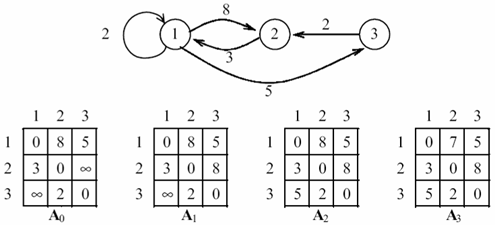
\includegraphics[width=13cm]{pic/45_02.png}

\end{figure}

\begin{lstlisting}[label=code:fl,caption=Опис функції алгоритму Флойда]
  // Опис функції алгоритму Флойда
 void Floyd (int n, int ** Graph, int ** ShortestPath) {
   int i, j, k;
   int Max_Sum = 0;
   for (i = 0; i <n; i ++)
     for (j = 0; j <n; j ++)
       Max_Sum + = ShortestPath [i] [j];
   for (i = 0; i <n; i ++)
     for (j = 0; j <n; j ++)
       if (ShortestPath [i] [j] == 0 && i! = j) 
         ShortestPath [i] [j] = Max_Sum;
   for (k = 0; k <n; k ++)
     for (i = 0; i <n; i ++)
       for (j = 0; j <n; j ++)
         if ((ShortestPath [i] [k] + ShortestPath [k] [j]) < 
              ShortestPath [i] [j])
           ShortestPath [i] [j] = ShortestPath [i] [k] + 
             ShortestPath [k] [j];
 } 
\end{lstlisting}
Зауважимо, що якщо граф неорієнтовний, то всі матриці, одержувані в результаті перетворень симетричні і, отже, досить вираховуватимуть тільки елементи, розташовані вище головної діагоналі.

Якщо граф представлений матрицею суміжності, то час виконання цього алгоритму має порядок O (n 3), оскільки в ньому присутні вкладені одна в одного три циклу. 


\subsection{Переборні алгоритми}

Переборні алгоритми по суті своїй є алгоритмами пошуку, як правило, пошуку оптимального рішення. При цьому рішення конструюється поступово. У цьому випадку зазвичай говорять про перебір вершин дерева варіантів. Вершинами такого графа будуть проміжні або кінцеві варіанти, а ребра вказуватимуть шляху конструювання варіантів.

Розглянемо Переборні алгоритми, засновані на методах пошуку в графі, на прикладі задачі знаходження найкоротшого шляху в лабіринті.

Постановка завдання.

Лабіринт, що складається з прохідних і непрохідних клітин, заданий матрицею A розміром mxn. Елемент матриці A [i, j] = 0, якщо клітина (i, j) прохідна. В іншому випадку $A_{[i, j]} = \infty $.

Потрібно знайти довжину найкоротшого шляху з клітини (1, 1) в клітину (m, n).

Фактично дана матриця суміжності (тільки в ній нулі замінені нескінченності, а одиниці - нулями). Лабіринт являє собою граф.

Вершинами дерева варіантів в даній задачі є шляхи, що починаються в клітці (1, 1). Ребра - показують хід конструювання цих шляхів і з'єднують два шляхи довжини k і k + 1, де другий шлях виходить з першого додаванням до шляху ще одного ходу.

Перебір з поверненням

Даний метод заснований на методі пошуку в глибину. Перебір з поверненням вважають методом проб і помилок ("спробуємо сходити в цю сторону: не вийде - повернемося і спробуємо в іншу"). Так як перебір варіантів здійснюється методом пошуку в глибину, то доцільно під час роботи алгоритму зберігати поточний шлях в дереві. Цей шлях являє собою стек Way.

Також необхідний масив Dist, розмірність якого відповідає кількості вершин графа, який зберігає для кожної вершини відстань від неї до вихідної вершини.

Нехай поточної є деяка клітина (на початку роботи алгоритму - клітина (1, 1)). Якщо для поточної клітини є клітина-сусід Neighbor, відсутня в Way, в яку на цьому шляху ще не ходили, то додаємо Neighbor в Way і поточної клітці присвоюємо Neighbor, інакше витягти з Way.

Наведене вище опис дає чітко зрозуміти, чому цей метод називається перебором з поверненням. Поверненню тут відповідає операція "витягти з Way", яка зменшує довжину Way на 1.

Перебір закінчується, коли Way порожній і робиться спроба повернення назад. У цій ситуації повертатися вже нікуди (рис.~\ref{pic:45.3}).

Way є поточним шляхом, але в процесі роботи необхідно зберігати і оптимальний шлях OptimalWay.

Удосконалення алгоритму можна зробити наступним чином: не дозволяти, щоб довжина Way була більше або дорівнює довжині OptimalWay. У цьому випадку, якщо і буде знайдений якийсь варіант, він свідомо не буде оптимальним. Таке удосконалення в загальному випадку означає, що як тільки поточний шлях стане свідомо неоптимальним, треба повернутися назад. Дане поліпшення алгоритму дозволяє в багатьох випадках сильно скоротити перебір.
Демонстрація алгоритму перебору з поверненням

\begin{figure}
\caption{Демонстрація алгоритму перебору з поверненням}\label{pic:45.3}
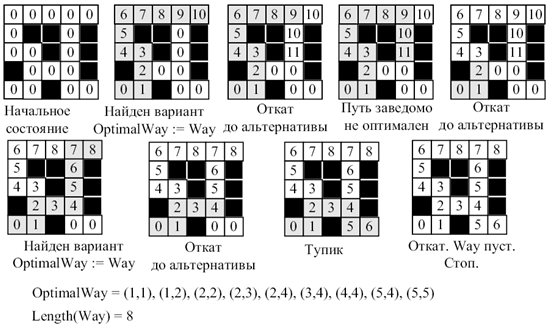
\includegraphics[width=13cm]{pic/45_03.png}
\end{figure}
\begin{lstlisting}
[label=code:pe,caption=Опис функції переборного алгоритму методом пошуку в глибину]
 / * Опис функції переборного алгоритму методом пошуку в глибину * /
void Backtracking (int n, int m, int ** Maze) {
  int Begin, End, Current;
  Begin = (n - 1) * m;
  End = m - 1;
  int * Way, * OptimalWay;
  int LengthWay, LengthOptimalWay;
  Way = new int [n * m];
  OptimalWay = new int [n * m];
  LengthWay = 0;
  LengthOptimalWay = m * n;
  for (int i = 0; i <n * m; i ++)
    Way [i] = OptimalWay [i] = -1;
  int * Dist;
  Dist = new int [n * m];
  for (int i = 0; i <n; i ++)
    for (int j = 0; j <m; j ++)
      Dist [i * m + j] = (Maze [i] [j] == 0? 0: -1);
  Way [LengthWay ++] = Current = Begin;
  while (LengthWay> 0) {
    if (Current == End) {
      if (LengthWay <LengthOptimalWay) {
        for (int i = 0; i <LengthWay; i ++)
          OptimalWay [i] = Way [i];
        LengthOptimalWay = LengthWay;
       }
      if (LengthWay> 0) Way [- LengthWay] = -1;
      Current = Way [LengthWay-1];
     }
    else {
      int Neighbor = -1;
      if ((Current / m - 1)> = 0 &&! Insert (Way, Current - m) &&
        (Dist [Current - m] == 0 || Dist [Current - m]> LengthWay)
        && Dist [Current] <LengthOptimalWay)
          Neighbor = Current - m;
       else 
        if ((Current% m - 1)> = 0 &&! Insert (Way, Current - 1) &&
          (Dist [Current - 1] == 0 || Dist [Current - 1]> LengthWay)
          && Dist [Current] <LengthOptimalWay)
            Neighbor = Current - 1;
         else 
          if ((Current% m + 1) <m &&! Insert (Way, Current + 1) &&
           (Dist [Current + 1] == 0 || Dist [Current + 1]> LengthWay)
          && Dist [Current] <LengthOptimalWay)
            Neighbor = Current + 1;
          else 
           if ((Current / m + 1) <n &&! Insert (Way, Current + m) &&
            (Dist [Current + m] == 0 || Dist [Current + m]> LengthWay)
           && Dist [Current] <LengthOptimalWay)
             Neighbor = Current + m;
      if (Neighbor! = -1) {
        Way [LengthWay ++] = Neighbor;
        Dist [Neighbor] = Dist [Current] + 1;
        Current = Neighbor;
       }
       else {
        if (LengthWay> 0) Way [- LengthWay] = -1;
        Current = Way [LengthWay-1];
       }
     }
   }
  if (LengthOptimalWay <n * m) 
    cout << endl << "Yes. Length way =" << LengthOptimalWay << endl;
  else cout << endl << "No" << endl;
 } 
\end{lstlisting}


\subsection{Хвильовий алгоритм}

Цей переборний алгоритм, який заснований на пошуку в ширину, складається з двох етапів:
\begin{itemize}
\item поширення хвилі;
\item зворотний хід.
\end{itemize}
 
Поширення хвилі і є власне пошук в ширину, при якому клітини позначаються номером кроку методу, на якому клітина відвідується. При зворотному ході, починаючи з кінцевої вершини, йде відновлення шляху, по якому в неї потрапили шляхом включення до нього клітин з мінімальною позначкою (рис.~\ref{pic:45.4}). Важливою особливістю є те, що відновлення починається з кінця (з початку воно найчастіше неможливо).
Демонстрація хвильового алгоритму

\begin{figure}
\caption{Демонстрація хвильового алгоритму}\label{pic:45.4}
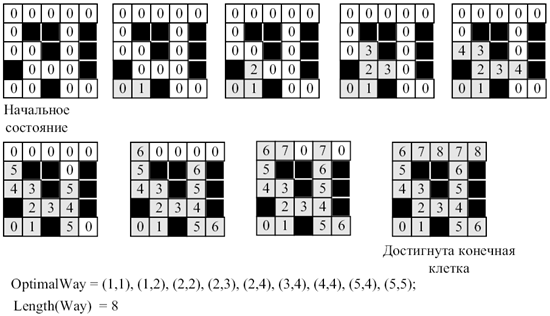
\includegraphics[width=13cm]{pic/45_04.png}
\end{figure}


Зауважимо, що перебір методом пошуку в ширину в порівнянні з перебором з поверненням, як правило, вимагає більше допоміжної пам'яті, яка необхідна для зберігання інформації, щоб побудувати шлях при зворотному ході і помітити відвідані вершини. Однак він працює швидше, оскільки абсолютно виключається відвідування однієї і тієї ж клітини більш ніж один раз.

\section{Приклади обчислень}
\nopagebreak[4]




\subsection*{Контрольні запитання}
\nopagebreak[4]
\begin{enumerate}
\item ?
\end{enumerate}




%\chapter{Використання багаторозгалужених дерев}
\nopagebreak[4]
\section*{Мета роботи}

\nopagebreak[4]
\section{Вступ}
\nopagebreak[4]


\section{Ключові терміни}
\nopagebreak[4]




\section{Розширені теоретичні відомості}
\nopagebreak[4]




\section{Приклади обчислень}
\nopagebreak[4]




\subsection*{Контрольні запитання}
\nopagebreak[4]
\begin{enumerate}
\item ?
\end{enumerate}




%\chapter{Алгоритми сортування}


\nopagebreak[4]
\section{Вступ}
\nopagebreak[4]
\textbf{Алгоритмом сортування} називається алгоритм для впорядкування деякого безлічі елементів. Зазвичай під алгоритмом сортування подразумевают алгоритм упорядкування безлічі елементів за зростанням або спаданням.

У разі наявності елементів з однаковими значеннями, у впорядкованій послідовності вони розташовуються поруч один за одним у будь-якому порядку. Однак іноді буває корисно зберігати первісний порядок елементів з однаковими значеннями.

Алгоритми сортування мають велике практичне застосування. Їх можна зустріти там, де мова йде про обробку та зберіганні великих обсягів інформації. Деякі завдання обробки даних вирішуються простіше, якщо дані заздалегідь впорядкувати.

\section{Ключові терміни}
\nopagebreak[4]




\section{Розширені теоретичні відомості}
\nopagebreak[4]
В алгоритмах сортування лише частина даних використовується як ключ сортування. Ключем сортування називається атрибут (або декілька атрибутів), за значенням якого визначається порядок елементів. Таким чином, при написанні алгоритмів сортувань масивів слід врахувати, що ключ повністю або частково збігається з даними.

Практично кожен алгоритм сортування можна розбити на 3 частини:
\begin{enumerate}
\item порівняння, визначальне впорядкованість пари елементів;
\item перестановку, змінюють місце пару елементів;
\item власне сортують алгоритм, який здійснює порівняння і перестановку елементів до тих пір, поки всі елементи множини не будуть впорядковані.
\end{enumerate}

\subsection{Оцінка алгоритмів сортування}

Жодна інша проблема не породила такої кількості найрізноманітніших рішень, як завдання сортування. Універсального, найкращого алгоритму сортування на даний момент не існує. Проте, маючи приблизні характеристики вхідних даних, можна підібрати метод, який працює оптимальним чином. Для цього необхідно знати параметри, за якими буде проводитися оцінка алгоритмів.

\textbf{Час сортування} - основний параметр, що характеризує швидкодію алгоритму.

\textbf{Пам'ять} - один з параметрів, який характеризується тим, що ряд алгоритмів сортування вимагають виділення додаткової пам'яті під тимчасове зберігання даних. При оцінці використовуваної пам'яті не враховуватиметься місце, яке займає вихідний масив даних і незалежні від вхідної послідовності витрати, наприклад, на зберігання коду програми.

\textbf{Стійкість} - це параметр, який відповідає за те, що сортування не змінює взаємного розташування рівних елементів.

\textbf{Природність поведінки} - параметр, якій вказує на ефективність методу при обробці вже відсортованих, або частково відсортованих даних. Алгоритм поводиться природно, якщо враховує цю характеристику вхідної послідовності і працює краще.

\subsection{Класифікація алгоритмів сортувань}

Все розмаїття і різноманіття алгоритмів сортувань можна класифікувати за різними ознаками, наприклад, по стійкості, по поведінці, по використанню операцій порівняння, за потреби в додатковій пам'яті, по потреби в знаннях про структуру даних, що виходять за рамки операції порівняння, та інші.

Найбільш докладно розглянемо класифікацію алгоритмів сортування за сферою застосування. У даному випадку основні типи впорядкування діляться наступним чином.

\textbf{Внутрішнє сортування} - це алгоритм сортування, який в процесі упорядкування даних використовує тільки оперативну пам'ять (ОЗП) на комп'ютері. Тобто оперативної пам'яті достатньо для завантаження в неї сортованого масиву даних з довільним доступом до будь-якій комірці і власне для виконання алгоритму. Внутрішня сортування застосовується у всіх випадках, за винятком однопрохідного зчитування даних і однопрохідної записи відсортованих даних. Залежно від конкретного алгоритму та його реалізації дані можуть сортуватися в тій же області пам'яті, або використовувати додаткову оперативну пам'ять.

\textbf{Зовнішнє сортування} - це алгоритм сортування, який при проведенні упорядкування даних використовує зовнішню пам'ять, як правило, жорсткі диски. Зовнішня сортування розроблена для обробки великих списків даних, які не поміщаються в оперативну пам'ять. Звернення до різних носіям накладає деякі додаткові обмеження на даний алгоритм: доступ до носія здійснюється послідовним чином, тобто в кожен момент часу можна вважати або записати тільки елемент, наступний за поточним; обсяг даних не дозволяє їм розміститися в ОЗУ.

Внутрішнє сортування є базовою для будь-якого алгоритму зовнішньої сортування - окремі частини масиву даних сортуються в оперативної пам'яті і за допомогою спеціального алгоритму зчіплюються в один масив, упорядкований по ключу.







%\chapter{Алгоритми внутрішнього сортування}
\nopagebreak[4]
\section*{Мета роботи}

\nopagebreak[4]
\section{Вступ}
\nopagebreak[4]


\section{Ключові терміни}
\nopagebreak[4]




\section{Розширені теоретичні відомості}
\nopagebreak[4]




\section{Приклади обчислень}
\nopagebreak[4]




\subsection*{Контрольні запитання}
\nopagebreak[4]
\begin{enumerate}
\item ?
\end{enumerate}




%\chapter{Алгоритми зовнішнього сортування}


\nopagebreak[4]
\section{Вступ}
\nopagebreak[4]
\textbf{Зовнішнє сортування} - сортування даних, розташованих на периферійних пристроях і не вміщаються в оперативну пам'ять, тобто коли застосувати одну з внутрішніх сортувань неможливо. Варто відзначити, що внутрішня сортування значно ефективніше зовнішньої, так як на звернення до оперативної пам'яті витрачається набагато менше часу, ніж до магнітних дисків, стрічок і т.п.

Найбільш часто зовнішнє сортування використовується в СУБД.

Дані, що зберігаються на зовнішніх пристроях, мають великий обсяг, що не дозволяє їх цілком перемістити в оперативну пам'ять, відсортувати з використанням одного з алгоритмів внутрішнього сортування, а потім повернути їх на зовнішній пристрій. У цьому випадку здійснювалося б мінімальну кількість проходів через файл, тобто було б однократне читання і однократна запис даних. Однак на практиці доводиться здійснювати читання, обробку і запис даних у файл по блоках, розмір яких залежить від операційної системи та наявного обсягу оперативної пам'яті, що призводить до збільшення числа проходів через файл і помітного зниження швидкості сортування.

\section{Ключові терміни}
\nopagebreak[4]
\textbf{Зовнішнє сортування} - це сортування даних, які розташовані на зовнішніх пристроях і не вміщаються в оперативну пам'ять.

\textbf{Фаза} - це дії по одноразовій обробці всієї послідовності елементів.

\textbf{Серія (упорядкований відрізок)} - це послідовність елементів, що упорядкована по ключу. Кількість елементів в серії називається довжиною серії.

\textbf{Двофазне сортування} - це сортування, в якому окремо реалізується дві фази: розподіл і злиття. 

\textbf{Однофазне сортування} - це сортування, в якому об'єднані фази розподілу і злиття в одну.

\textbf{Двоколійним злиттям} називається сортування, в якому дані розподіляються на два допоміжних файли. 

\textbf{Багатоколійним злиттям} називається сортування, в якому дані розподіляються на N (N> 2) допоміжних файлів.



\section{Розширені теоретичні відомості}
\nopagebreak[4]

\subsection{Сортування простим злиттям}

Одне з сортувань на основі злиття називається простим злиттям.

Алгоритм сортування простим злиття є найпростішим алгоритмом зовнішньої сортування, заснований на процедурі злиття серією.

У даному алгоритмі довжина серій фіксується на кожному кроці. У вихідному файлі всі серії мають довжину 1, після першого кроку вона дорівнює 2, після другого - 4, після третього - 8, після k-го кроку - 2k.

Алгоритм сортування простим злиттям

\begin{enumerate}
\item Вихідний файл f розбивається на два допоміжних файлу f1 і f2.

\item Допоміжні файли f1 і f2 зливаються в файл f, при цьому поодинокі елементи утворюють впорядковані пари.

\item Отриманий файл f знову обробляється, як зазначено в кроках 1 і 2. При цьому впорядковані пари переходять у впорядковані четвірки.

\item Повторюючи кроки, зливаємо четвірки в вісімки і т.д., кожен раз подвоюючи довжину злитих послідовностей до тих пір, поки не буде впорядкований цілком весь файл (рис.~\ref{f:sort1}).
\end{enumerate}

\begin{figure}
\caption{Демонстрація сортування двоколійному двофазним простим злиттям}\label{f:sort1}
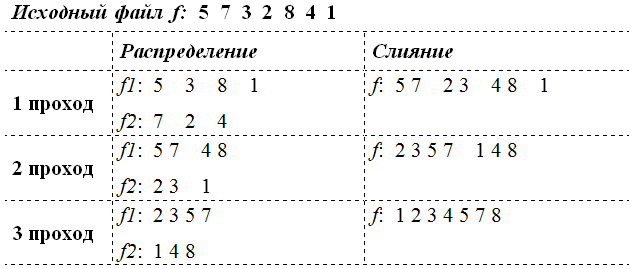
\includegraphics[width=13cm]{pic/43_01.png}

\end{figure}

Після виконання i проходів отримуємо два файли, що складаються з серій довжини 2i. Закінчення процесу відбувається при виконанні умови $2^i \geq n$. Отже, процес сортування простим злиттям вимагає порядку $O (\log n)$ проходів за даними.

Ознаками кінця сортування простим злиттям є наступні умови:

\begin{enumerate}
\item довжина серії не менша кількість елементів у файлі (визначається після фази злиття);
\item кількість серій рівно 1 (визначається на фазі злиття).
\item при однофазному сортуванні другий за рахунком допоміжний файл після розподілу серій залишився порожнім.
\end{enumerate}

Приклад програмної реалізації надано у додатку \ref{code:sort111};

\section{Приклади обчислень}
\nopagebreak[4]







%\chapter{Характеристика алгоритмів порівняння методів сортування}
\nopagebreak[4]
\section*{Мета роботи}

\nopagebreak[4]
\section{Вступ}
\nopagebreak[4]


\section{Ключові терміни}
\nopagebreak[4]




\section{Розширені теоретичні відомості}
\nopagebreak[4]




\section{Приклади обчислень}
\nopagebreak[4]




\subsection*{Контрольні запитання}
\nopagebreak[4]
\begin{enumerate}
\item ?
\end{enumerate}




\appendix
\makeatletter
\gdef\thechapter{\@Asbuk\c@chapter}
\makeatother
\def\chaptername{Додаток}


\chapter{Правила оформлення звіту}
\section{Титульна сторінка лабораторної роботи}
\input{ap01-00}
\section{Приклади блок-схем}
Правила виконання блок-схем задані наступними документами:
\begin{itemize}
\item ГОСТ 19.701-90. Схемы алгоритмов, программ, данных и систем. Условные обозначения и правила выполнения
\item ГОСТ 19.002-80. Схемы алгоритмов и программ. Правила выполнения
\item ГОСТ 19.003-80. Схемы алгоритмов и программ. Обозначения условные графические

\end{itemize}



%\include{ap02}
%\include{ap03}
%\include{ap04}
%\include{ap05}
%\include{ap06}
%\include{ap07}
%\include{ap08}
%\include{ap09}
%\include{ap10}
 
 



%% указываем класс документа
%\documentclass[twoside,8pt,a5paper,openany]{report}
\documentclass[twoside,12pt,a4paper,openany]{report}

% подключаем собственный стилевой файл
\usepackage{labstyle}
\usepackage{labstyle2}







\makeindex





\begin{document}


% указываем язык (для автоматической вставки слов, типа "Глава", "Содержание", "Литература", "рис." и пр.
\selectlanguage{ukrainian}



% подключаем файлы содержимого
\include{cover}
\include{ch00}
\include{ch01}
\include{ch02}
%\include{ch03}
%\include{ch04} 
%\include{ch05}
%\include{ch06}
%\include{ch07}
%\include{ch08}
%\include{ch09}
%\include{ch10}
\appendix
\makeatletter
\gdef\thechapter{\@Asbuk\c@chapter}
\makeatother
\def\chaptername{Додаток}


\include{ap01}
%\include{ap02}
%\include{ap03}
%\include{ap04}
%\include{ap05}
%\include{ap06}
%\include{ap07}
%\include{ap08}
%\include{ap09}
%\include{ap10}
 
 



%\input{all.ind}

\bibliographystyle{ugost2008l}
\bibliography{bibi}  




\end{document}


\bibliographystyle{ugost2008l}
\bibliography{bibi}  




\end{document}


\bibliographystyle{ugost2008l}
\bibliography{bibi}  




\end{document}


\bibliographystyle{ugost2008l}
\bibliography{bibi}  




\end{document}
